\documentclass[12pt,a4paper]{article}
\usepackage[warn]{mathtext}
\usepackage[utf8]{inputenc}
\usepackage[T2A]{fontenc}
\usepackage[english,russian]{babel}


\usepackage{indentfirst}
\usepackage{misccorr}

\usepackage{subcaption}
\captionsetup{compatibility=false}
\usepackage{wrapfig}
\usepackage{amsmath}
\usepackage{floatflt}
\usepackage{float}
\usepackage{amssymb}
\usepackage{color}
\usepackage{lscape}
\usepackage{hvfloat}
\usepackage{amsfonts}
\usepackage{euscript}
\usepackage{textcomp}
\usepackage{mathtext}
\usepackage{latexsym}
\usepackage{xcolor}
\usepackage{hyperref}
\usepackage{booktabs}
\usepackage[version =3]{mhchem}
\usepackage{commath}
\usepackage{gensymb}
\usepackage[normalem]{ulem}
\usepackage{fancyhdr}


\newcommand{\RomanNumeralCaps}[1]
    {\MakeUppercase{\romannumeral #1}}

\graphicspath{{pictures/}}

\definecolor{linkcolor}{HTML}{000BFF} % цвет ссылок
\definecolor{urlcolor}{HTML}{000BFF} % цвет гиперссылок
 
\ULdepth = 0.16em
 
\hypersetup{pdfstartview=FitH,  linkcolor=linkcolor,urlcolor=urlcolor, colorlinks=true} 
\graphicspath{{pictures/}}
\DeclareGraphicsExtensions{.png,.jpg, .jpeg}
\usepackage[left=20mm, top=20mm, right=20mm, bottom=20mm, footskip=10mm]{geometry}
\linespread{1.3}

\begin{document}
\begin{titlepage}
  \begin{center}
    \Large МОСКОВСКИЙ ФИЗИКО-ТЕХНИЧЕСКИЙ ИНСТИТУТ\\
    \large национальный исследовательский университет
    \vspace{0.5cm}
   
    \vspace{0.25cm}
 
    \vfill
 
    \vfill

    \large{Вопрос по выбору к экзамену по основам современной физики:}\\[2mm]
    
    {\LARGE Генератор гетеродина на основе\\
    распределённого джозефсоновского перехода}

    \vfill
    
\end{center}

\vfill
\vfill
\vfill

\begin{flushright}

    Выполнили студенты 3 курса ФФКЭ:\\
    Атепалихин Артемий Алексеевич, группа 854,\\
    Водзяновский Яромир Олегович, группа 852,\\
    инженеры лаб. 234 ИРЭ РАН

\end{flushright}
\bigskip


\vfill

\begin{center}
  Долгопрудный, 2021 г.
\end{center}
\end{titlepage}

\pagestyle{fancy} 
    \fancyhead[L]{Водзяновский Я.О}
    \fancyhead[R]{Основы современной физики}
    \fancyhead[C]{РДП}
    \fancyfoot[C]{ \noindent\rule{\textwidth}{0.4pt} \thepage }

\newpage

\tableofcontents

\newpage

\section{Основные понятия и аббривиатуры}

    \begin{itemize}
        \item SIS - superconductor-insulator-superconductor\\ (СИС - сверхпроводник-изолятор-сверхпроводник)
        \item FFO - flux-flow oscillator\\ (РДП - распределённый джозефсоновский переход)
        \item СВЧ - сверхвысокие частоты
        \item Эффект Джозефсона (стац.)
        \item Джозефсоновский переход
        \item Режим flux-flow
        \item Ступени Фиске
    \end{itemize}

\section{Описание работы}

\subsection{Задача исследования}
Основными целями являются:

    \begin{enumerate}
        \item Приведение краткого теоретического описания принципа работы РДП
        \item Демонстрирование результатов эксперементального исследования одного из изготовленных в ИРЭ им. В.А. Котельникова РАН образцов
    \end{enumerate}

\subsection{Общая информация}

Использующийся в качестве генератора гетеродина распределённый джозефсоновский переход является важнейшей частью одного из возможных вариантов устройств, способных излучать и принимать в ТГц и субТГц диапазонах, внимание к которым многократно возросло за последние пару десятилетий. Приёмники, работающие свыше нескольких сотен ГГц, крайне необходимы для целого ряда направлений современной науки: от медицины и биологии до аэрологии и астрофизики. Стоит отметить, что сказанное выше не является красивыми возможностями и грандиозными планами: сверхпроводниковые гетеродинные приёмники ТГц излучения уже довольно долго и очень активно используются в наземных, воздушных и космических миссиях (подр. - \cite{Kinev})
\:

\:

\newpage

\section{СИС - контакт}

В основе описываемого далее метода приёма СВЧ сигнала лежит \textit{джозефсоновский контакт} - два сверхпроводниковых элемента, имеющие слабую свзяь, которая в нашем случае организована путем нанесения тонкого слоя диэлектрика ($\pm 10$ нм) между ними. Схема СИС-контакта приведена на рисунке \ref{sis}.

    \begin{figure}[h]
            \begin{minipage}[h]{0.55\linewidth}
            \center{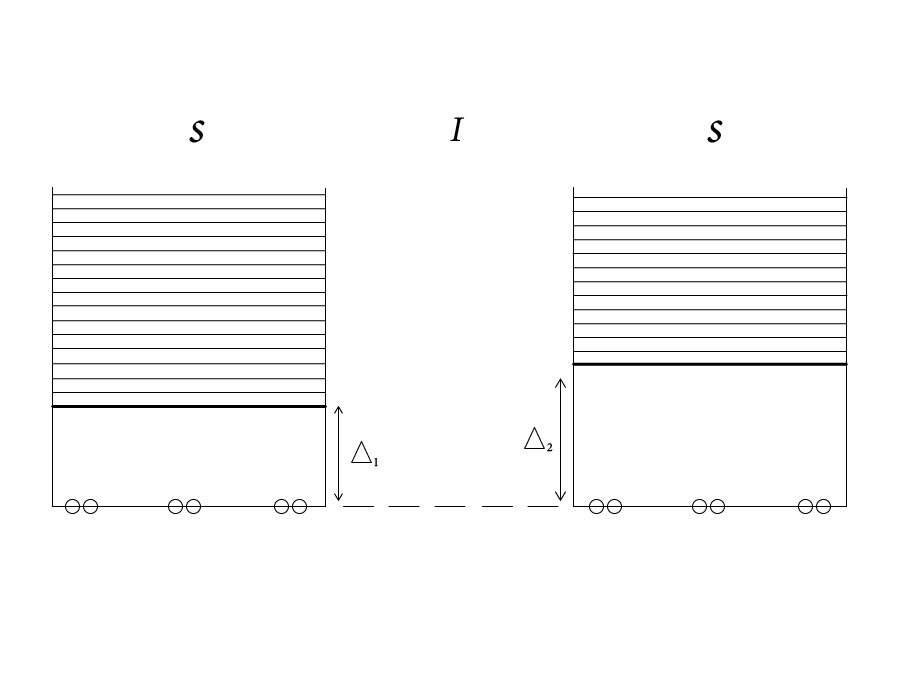
\includegraphics[width=0.95\linewidth]{sis a.png} \\ а) без приложенного напряжения;}
            \end{minipage}
        \hfill
            \begin{minipage}[h]{0.55\linewidth}
            \center{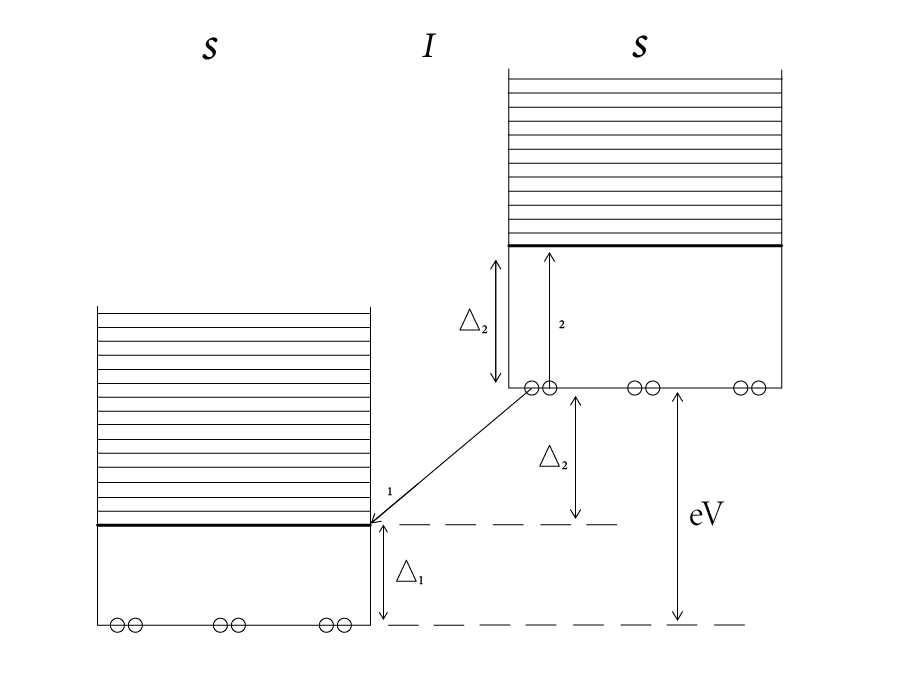
\includegraphics[width=0.95\linewidth]{sis b.png} \\ б) с приложенным напряжением.}
            \end{minipage}
        \caption{Энергетические диаграммы контакта SIS}
        \label{sis}
    \end{figure}

В случае слабой связи двух сверхпроводников кроме туннелирования
электронов, образовавшихся в результате разрыва куперовских пар, могут
туннелировать сами пары даже без приложенного напряжения. Такой поток зарядов
называется джозефсоновским током; его плотность определяется некоторой
константой $j_c$ и разницей фаз волновых функций куперовских пар в двух
сверхпроводниках. Данный эффект называется стационарным эффектом Джозефсона.

\newpage

\section{Принцип гетеродинирования}

\textbf{Гетеродинирование} - это процесс, в котором сильный монохроматический сигнал гетеродина (LO) и слабый интересующий сигнал (s) накладываются на детектор с нелинейной кривой ВАХ. Из-за нелинейности в смесителе генерируется много суммарных и разностных частот:

\begin{equation}
    |nF_{s} - mF_{LO}|
\end{equation}

\textbf{Смеситель} (в нашем случае) - трёх-портовое устройство, принимающее на вход исследуемый сигнал (s) и сигнал гетеродина (LO), а на выходе выдает промежуточный сигнал (IF). (рис. \ref{mixer})

\begin{figure}[H]
    \centering
    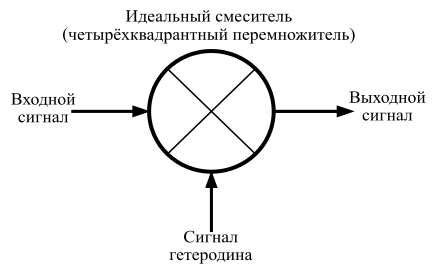
\includegraphics[scale = 0.5]{mixer.png}
    \caption{Схема смесителя}
    \label{mixer}
\end{figure}

Пусть сигналы s и LO выглядят следующим образом:

\begin{equation}
    V_{LO} = V_{LO} \sin{(2 \pi F_{LO}t)}, \;\; V_s = V_s \sin{(2 \pi F_s t)}
    \label{eq:he-signals}
\end{equation}

Будем полагать, что в SIS смесителе нелинейный ВАХ имеет слующую зависимость:
\begin{equation}
    I = a V^2
    \label{eq:sis-iv}
\end{equation}

Отсюда, путем подстановки суммы выражений (\ref{eq:he-signals}) в (\ref{eq:sis-iv}):

\begin{equation}
    I = a (V_s + V_{LO}) = \ldots + aV_sV_{LO} \left(\cos{[2\pi(F_s - F_{LO})t]} - \cos{[2\pi(F_s + F_{LO})t]} \right)
\end{equation}

Из уравнения выше видно, что ток детектора имеет спеткральные компоненты на частотах $F_s \pm F_{LO}$. Выходящий сигнал IF будет иметь амплитуду пропорциональную входящему сигналу s, но сниженным по частоте $F_{IF} = F_s - F_{LO}$.\par 

На рис. \ref{mixer} представлена иллюстрация принципа работы смесителя. Будут присутсвовать две полосы справа (Upper sideband) и слева (Lower sideband) от частоты гетеродина. 

\begin{figure}[H]
    \centering
    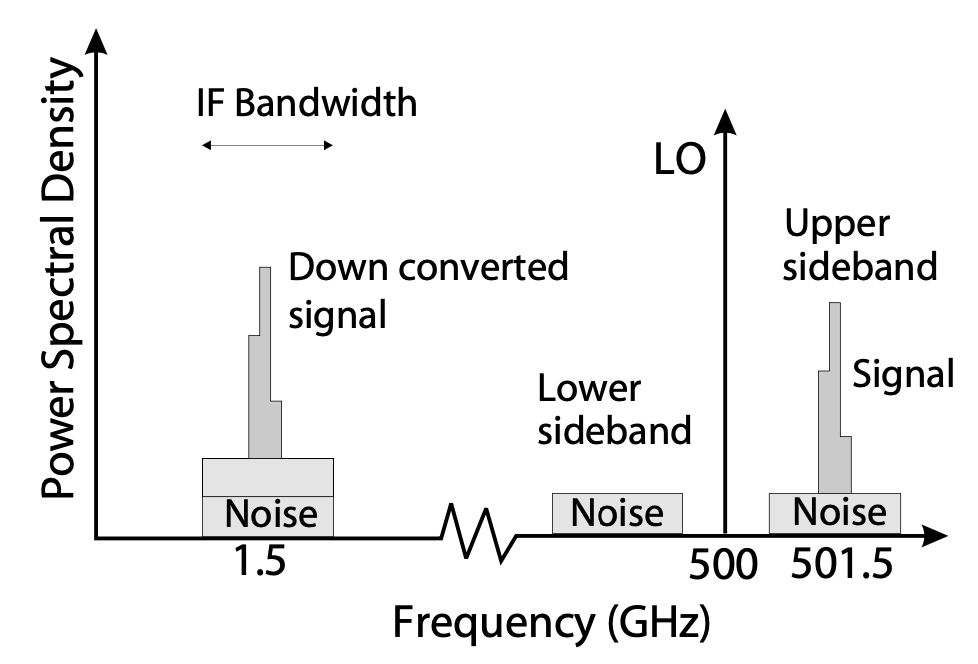
\includegraphics[scale = 0.7]{detect.png}
    \caption{Иллюстрация принципа гетеродинирования. $F_{LO} = 500 GHz, \; F_{IF} = 1.5 GHz$}
    \label{mixer}
\end{figure}

\begin{figure}[H]
    \centering
    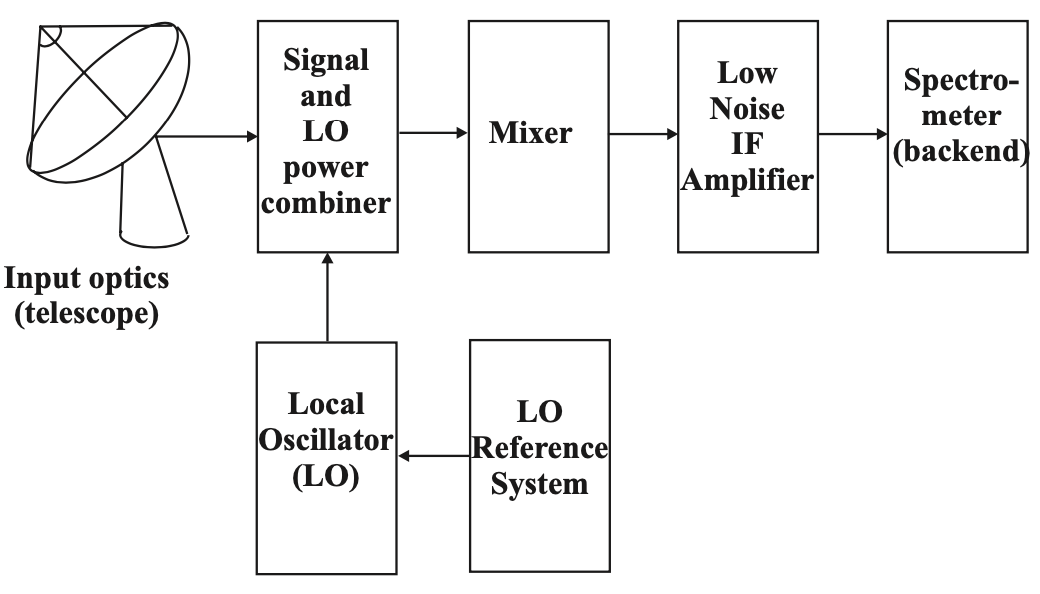
\includegraphics[scale = 0.8]{block-scheme.png}
    \caption{Блок схема полного процесса детектирования сигнала}
    \label{shem}
\end{figure}

\newpage

\section{Физика работы РДП}

\subsection{Общяя теория РДП}

В качестве РДП используются переходы на основе туннельных структур $Nb/AlO_x/Nb$ и $Nb/AlN/NbN$ геометрии «overlap» (перевод с англ. – частичное перекрытие, совмещение) с поперечным заданием тока смещения $I_B$. Характерная длина РДП составляет 300 – 700 мкм при ширине W от 3 до 20мкм. Величина критической плотности тока $j_c$ лежит в диапазоне $2-10кA/cм^2$, что соответствует джозефсоновской глубине проникновения магнитного поля $\lambda_J \approx$ 8 - 2 мкм. Для структур $Nb/AlO_x/Nb$ «щелевое напряжение» $V_g \approx$ 2.8 мВ, в то время как для структур $Nb/AlN/NbN$ $V_g \approx$ 3.7мВ при Т=4.2К. \par 

В РДП под действием силы Лоренца, создаваемой магнитным полем и транспортным током, называемого током смещения $I_B$, движутся джозефсоновские вихри – флаксоны. Каждый такой вихрь содержит квант магнитного потока $\varPhi_0 = h/2e$, а его размер составляет порядка $2\lambda_J$ вдоль оси перехода и $2\lambda_L$ в перпендикулярном плоскости туннельного слоя направлении, где $\lambda_L$ - глубина лондоновского проникновения поля в электроды. Типичное значение $\lambda_L$ для пленок ниобия, используемое в расчетах, составляет 90 нм. 

\begin{figure}[H]
    \centering
    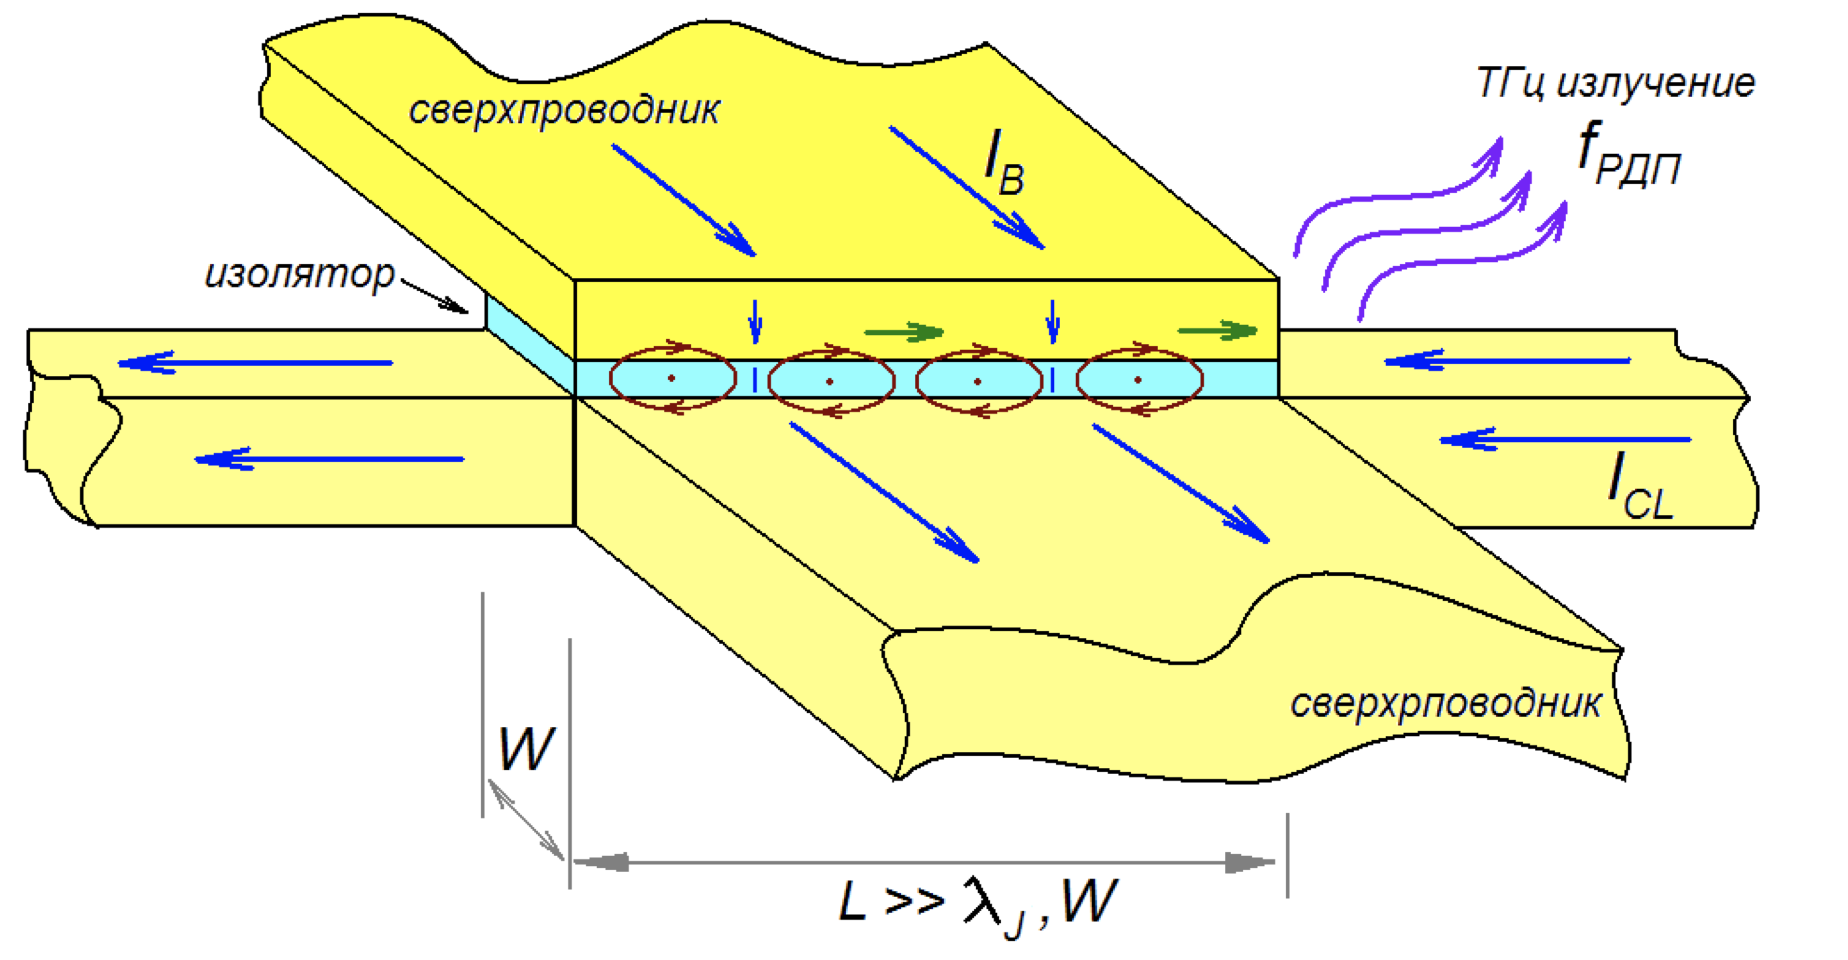
\includegraphics[scale = 0.5]{FFO.png}
    \caption{Геометрия РДП}
    \label{FFO}
\end{figure}

Для создания магнитного поля на концах РДП используется линия управления магнитным полем с током $I_{CL}$, конструктивно представляющая собой нижний сверхпроводящий электрод из ниобия (рис. \ref{FFO}). Кванты магнитного потока, двигаясь по переходу под действием силы Лоренца, достигают края и излучают электромагнитную волну в микрополосковую линию, соединенную с переходом через трансформатор импеданса, который необходим для согласования микрополосковой линии и имеющего низкий импеданс РДП. Таким образом, переход при напряжении $V_{РДП}$ генерирует электромагнитные колебания с частотой $f_{РДП}$, определяемой соотношением Джозефсона (\ref{eq:jos-eq}) (порядка 483.6ГГц/мВ).
\begin{equation}
    h f_{\text{РДП}} = 2 e V_{\text{РДП}}
    \label{eq:jos-eq}
\end{equation}
Скорость и плотность потока флаксонов, и, следовательно, мощность и частоту излучения можно перестраивать путем изменения тока смещения или/и магнитного поля.

\subsection{Режимы работы}

Из-за особенностей материалов изготовления образцов область приёма сигнала ограничена $\sim150$ ГГц снизу и $\sim700$ ГГц сверху, причём в разных диапазонах приём осуществляется разными механизмами. \par 

Будем пологать, что внешнее магнитное поле $H > H_{c1}$
\begin{equation}
   H_{c1} = \frac{\varPhi_0}{\pi \Lambda \lambda_J}, 
\end{equation}
где $\Lambda$ - магнитная толщина барьера. \par

Регулировать режим работы будет параметр затухания $\alpha$, который имеет физический смысл нормальной проводимости туннельного барьера на единицу длины перехода. На ВАХ (рис. \ref{FFO-iv}) видно, что есть граничное напряжение $V_{JSC}$ в котором параметр $\alpha$ испытывает скачек и режим работы меняется.

\begin{figure}[H]
    \centering
    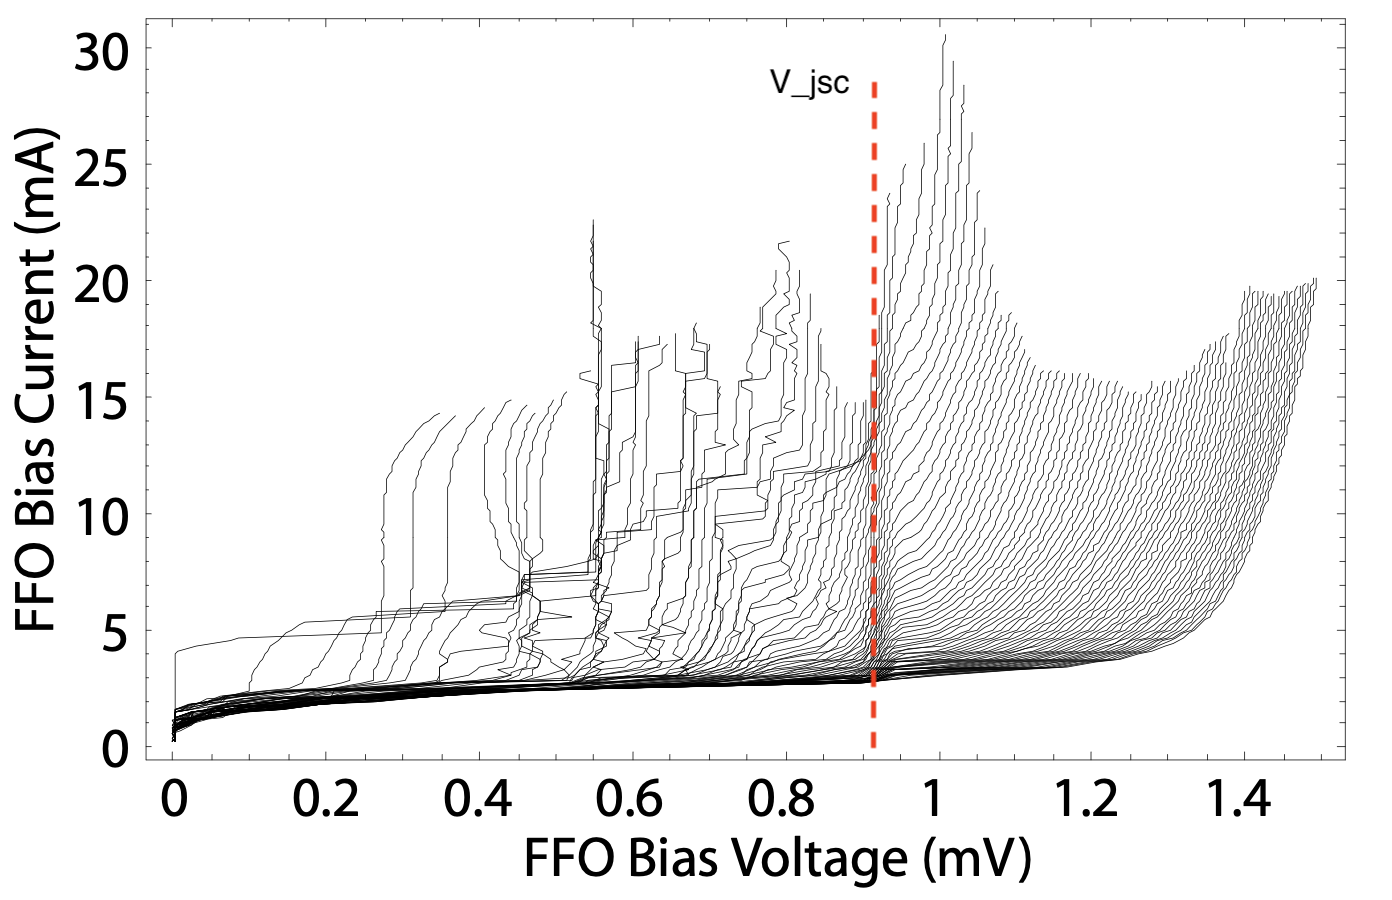
\includegraphics[scale = 0.5]{FFO_iv.png}
    \caption{Пример ВАХ РДП, с обозначенным напряжением $V_{JSC}$ скачка параметра $\alpha$}
    \label{FFO-iv}
\end{figure}

Рассмотрим следующие случаи:

\subsubsection{Генерация ступенями Фиске}

Рассмотрим ситуацию, когда напряжение  $V < V_{JSC}$. \par 

При столкновении кванта магнитного потока с краем перехода часть электромагнитного излучения отражается обратно, при этом отраженная волна может в случае малого $\alpha$ достигнуть противоположного края. Тогда возникают стоячие волны, которые при определенных резонансных частотах облегчают вхождение в переход флаксонов, в результате чего ВАХ имеют ярко
выраженную резонансную структуру. Чем меньше затухание, тем острее резонансные пики и круче структура ВАХ, которую называют ступенями Фиске.
Часть флаксонов покидают переход, они вызывают изменение тока и напряжения таким образом, что их энергия конвертируется в Э-М излучение.

См. \cite{Barychev}

\subsubsection{Режим flux-flow}

Рассмотрим ситуацию, когда напряжение  $V > V_{JSC}$. \par
Форма ВАХ становится более плавной, наклон кривых уменьшается (дифференциальное сопротивление увеличивается), что облегчает непрерывную перестройку рабочей частоты РДП, но увеличивает его полосу излучения. Такой режим является истинным «флакс-флоу» режимом (от англ. Flux- flow - вязкий поток вихрей), описываемым в работах без учета стоячей волны, т.е. где не был реализован резонансный режим.

См. \cite{Barychev}

\subsection{Накачка детектора}

После получения высокочастотной электромагнитной волны необходимо её принять. Для передачи сигнала была сконструирована специальная схема, показанная на рисунке \ref{cpl}. Детектором в ней является сосредоточенный джозефсоновский переход - обычный СИС.

\begin{figure}[H]
    \centering
    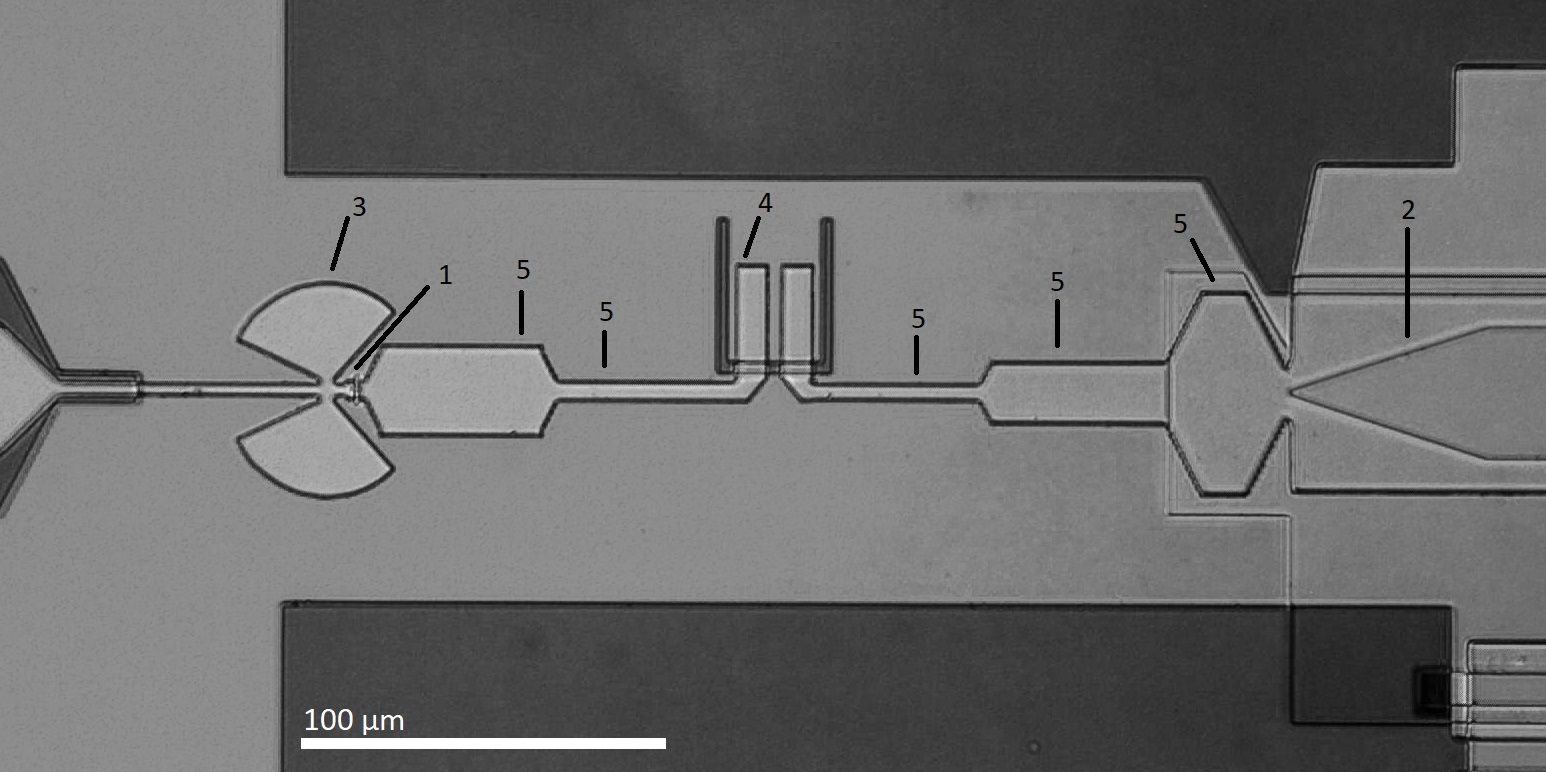
\includegraphics[scale = 0.8]{real-scheme.jpg}
    \caption{Схема микрополосковой линии для исследования характеристик РДП. 1 - SIS переход; 2 - РДП; 3 - Radial stab; 4 - DC-break; 5 - микрополосковые линии.}
    \label{cpl}
\end{figure}

Электромагнитная волна, пришедшая к детектору, воздействует на электроны в валентной зоне верхнего сверхпроводящего электрода, см. рис. \ref{hf}.
Получивший энергию {$\hbar \omega$} электрон теперь способен преодолеть барьер {$\Delta_1 + \Delta_2$} даже без приложенного напряжения.

\begin{figure}[H]
    \centering
    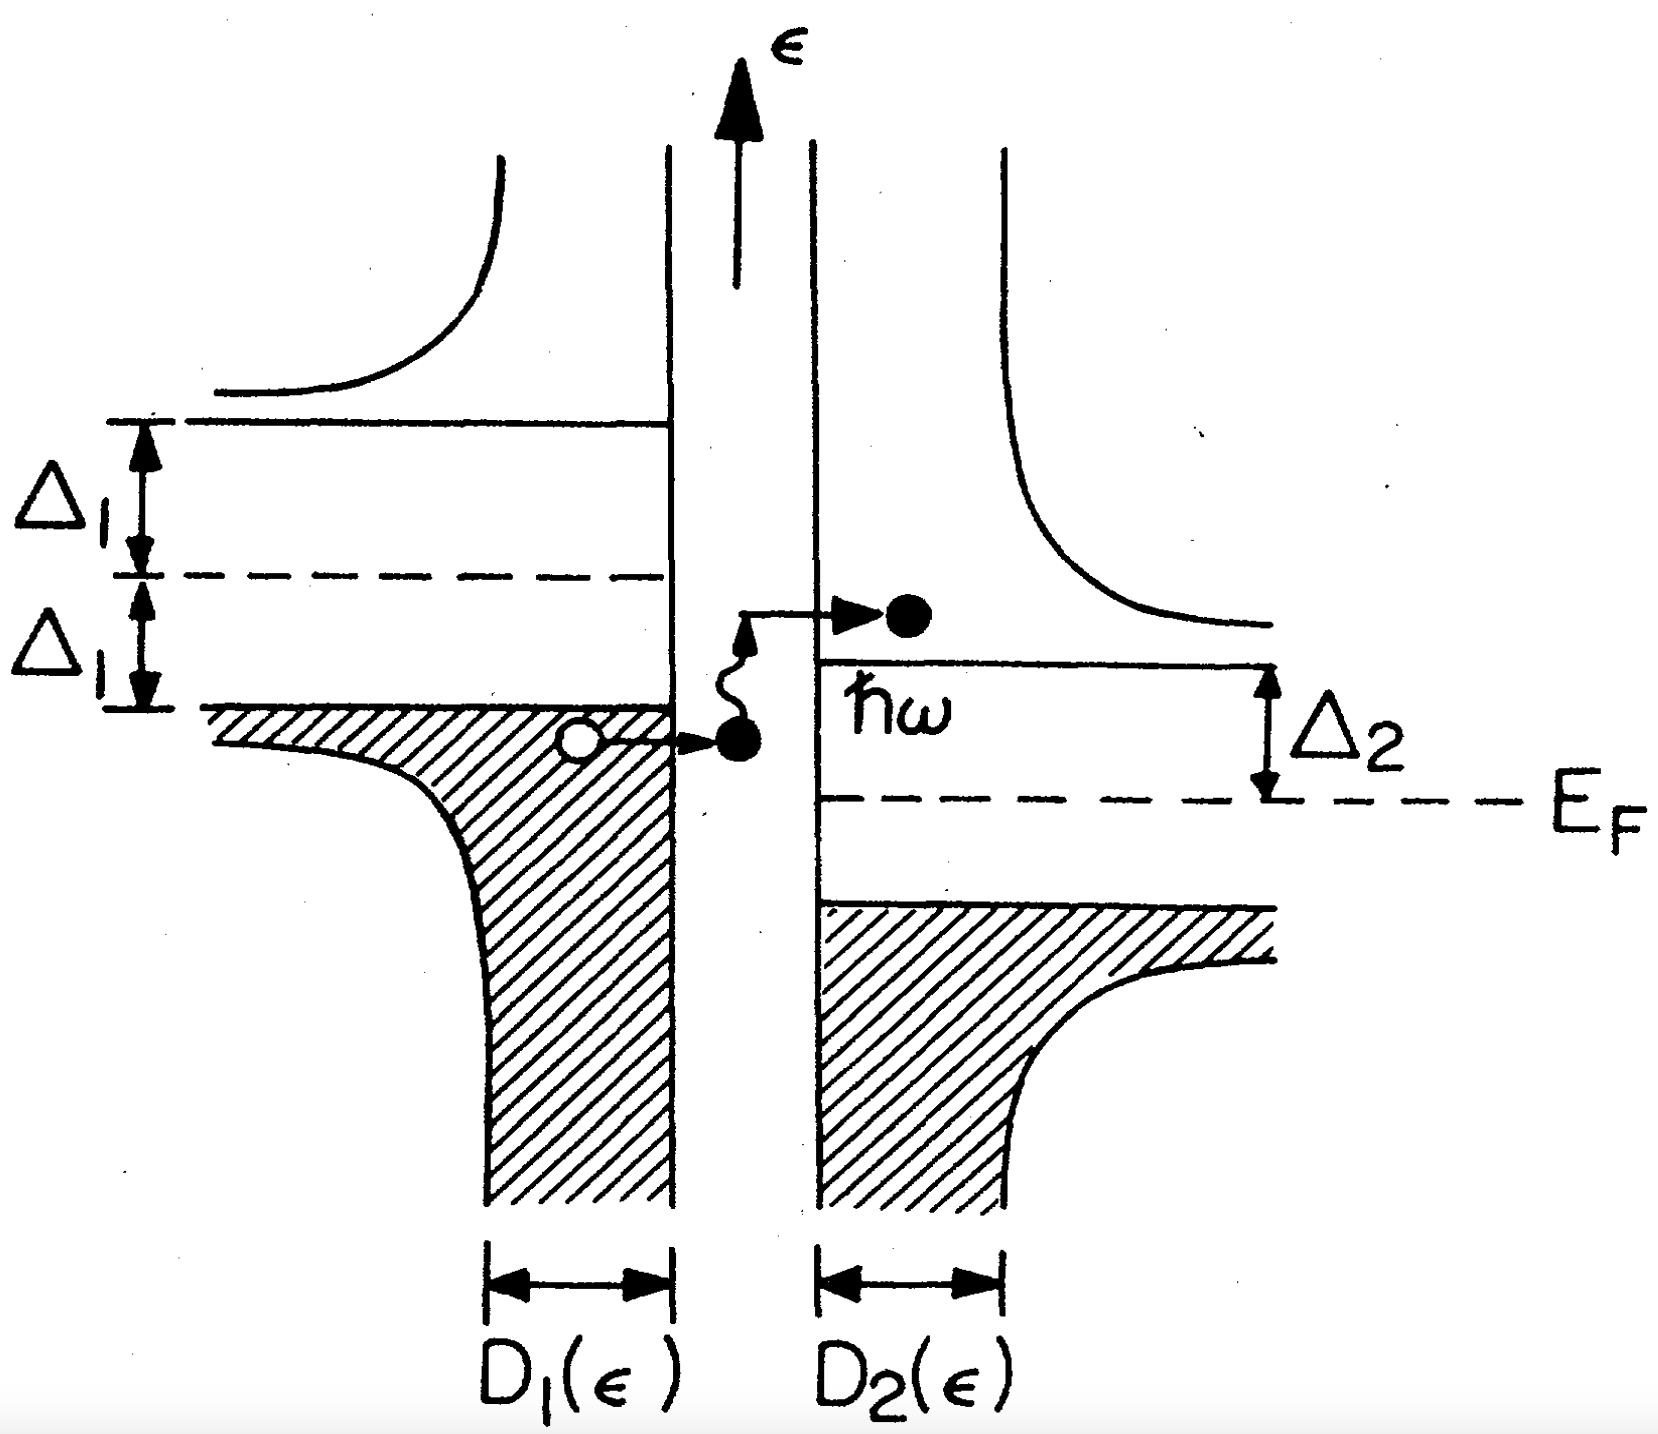
\includegraphics[scale = 0.27]{Diagram.png}
    \caption{Энергетическая диаграмма SIS перехода}
    \label{hf}
\end{figure}

В общем случае условие туннелирования электрона из валентной зоны одного сверхпроводника в зону проводимости второго выглядит следующим образом (см. \cite{Tucker}):

\begin{equation}
    eV + \hbar \omega \geq \Delta_1 + \Delta_2
\end{equation}

Результат такого эффекта отражается на ВАХ СИС-перехода (рисунок \ref{sis-iv}): сплошная кривая является ненакаченной характеристикой, пунктирная - под воздействием электромагнитного сигнала частотой {$\omega$}. Джозефсоновский ток подавлен магнитным полем.

\begin{figure}[H]
    \centering
    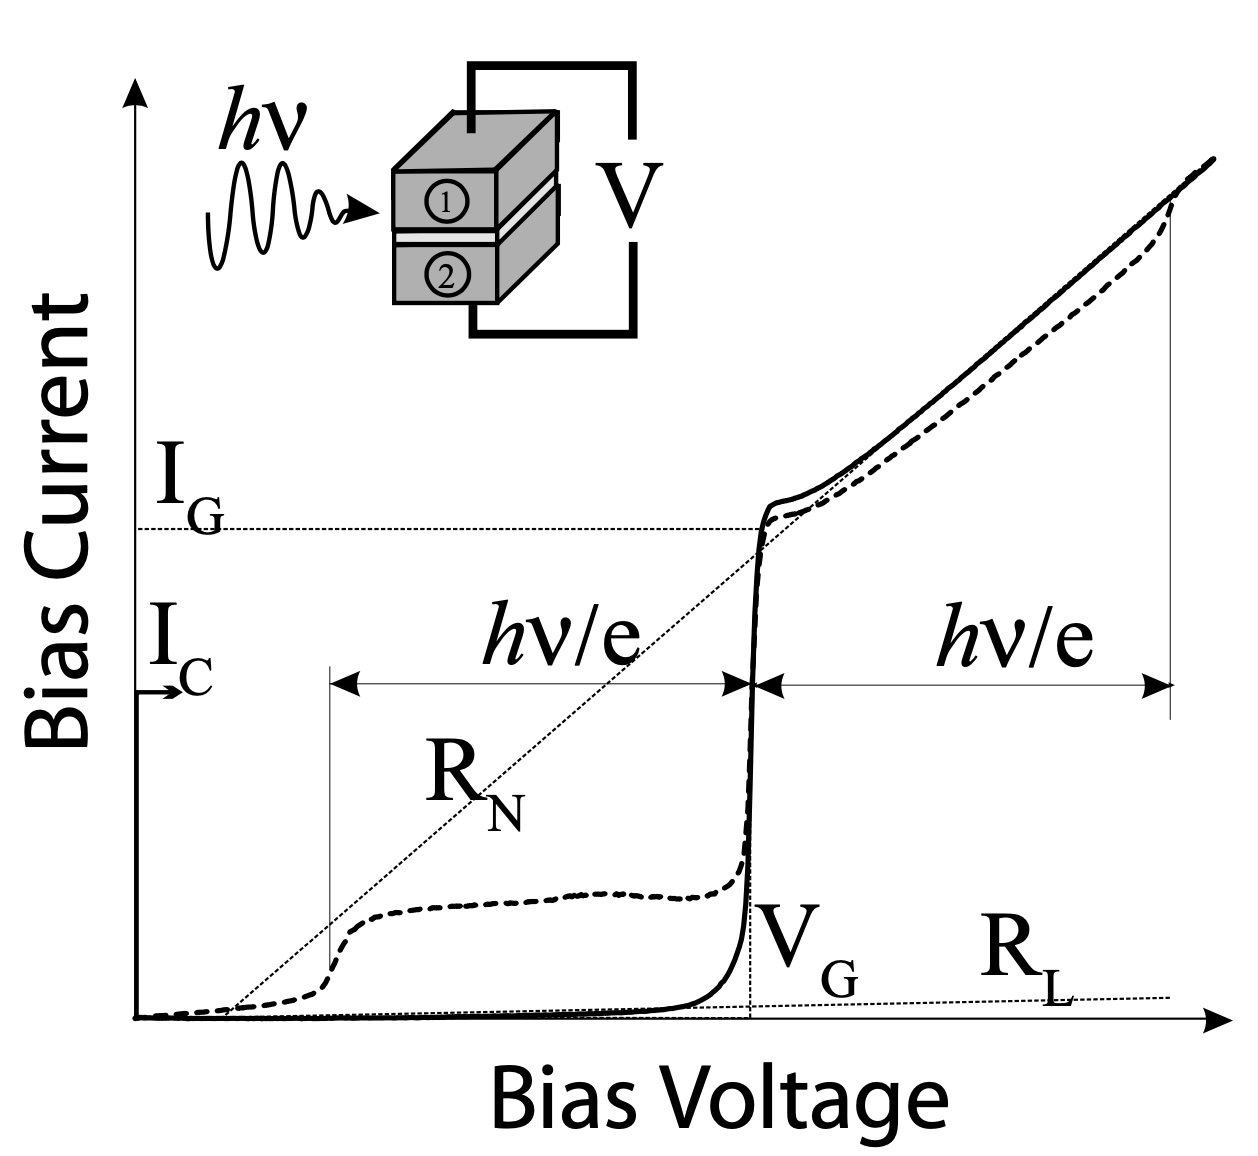
\includegraphics[scale = 0.4]{i-v-curve.png}
    \caption{ВАХ SIS-перехода}
    \label{sis-iv}
\end{figure}

%можно пару слов о том что мы в итоге дальше с этим делаем, потому что вопрос более чем резонный

\newpage

\section{Эксперимент}

\subsection{Установка}

Для осуществления перехода ниобиевых плёнок в сверхпроводящий режим необхоимо охладить образец (рис. \ref{chip}.а) как минимум до 9,25К ({$T_C$} Nb). Для этого чип помещается в специальный держатель (рис. \ref{chip}.б), который с помощью соединительных проводов (рис. \ref{exp}.а) подключает образец к измерительным блокам необходимым образом. Далее в защитном корпусе плата с чипом опускается в дьюар с гелием (рис. \ref{ust}, \ref{exp}.б), где происходит охлаждение до 4,2К, т.к. это температура кипения гелия. После этого можно приступать к измерениям.

\begin{figure}[H]
    \begin{center}
    \center{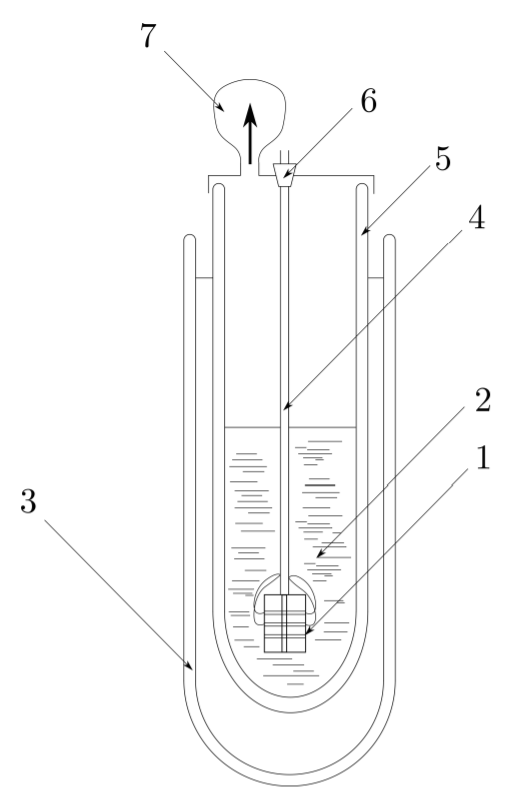
\includegraphics[scale=0.7]{ustanovka.png}}
    \caption{схема измерительной установки.}
    \label{ust} 
    \end{center}
\end{figure}

 1 - цилиндр с образцом, помещённый в жидкий гелий;
 
 2 - гелий;
 
 3 - внешняя стенка сосуда (дьюара);
 
 4 - т.н. ``макалка'' - металиическая трубка с соединительными проводами внутри;
 
 5 - внутренняя стенка сосуда, отделена от внешней вакуумом;
 
 6 - фиксатор глубины погружения цилиндра;
 
 7 - индикатор испарения гелия (резиновая груша).


\begin{figure}[H]
    \begin{minipage}[h]{0.5\linewidth}
        \center{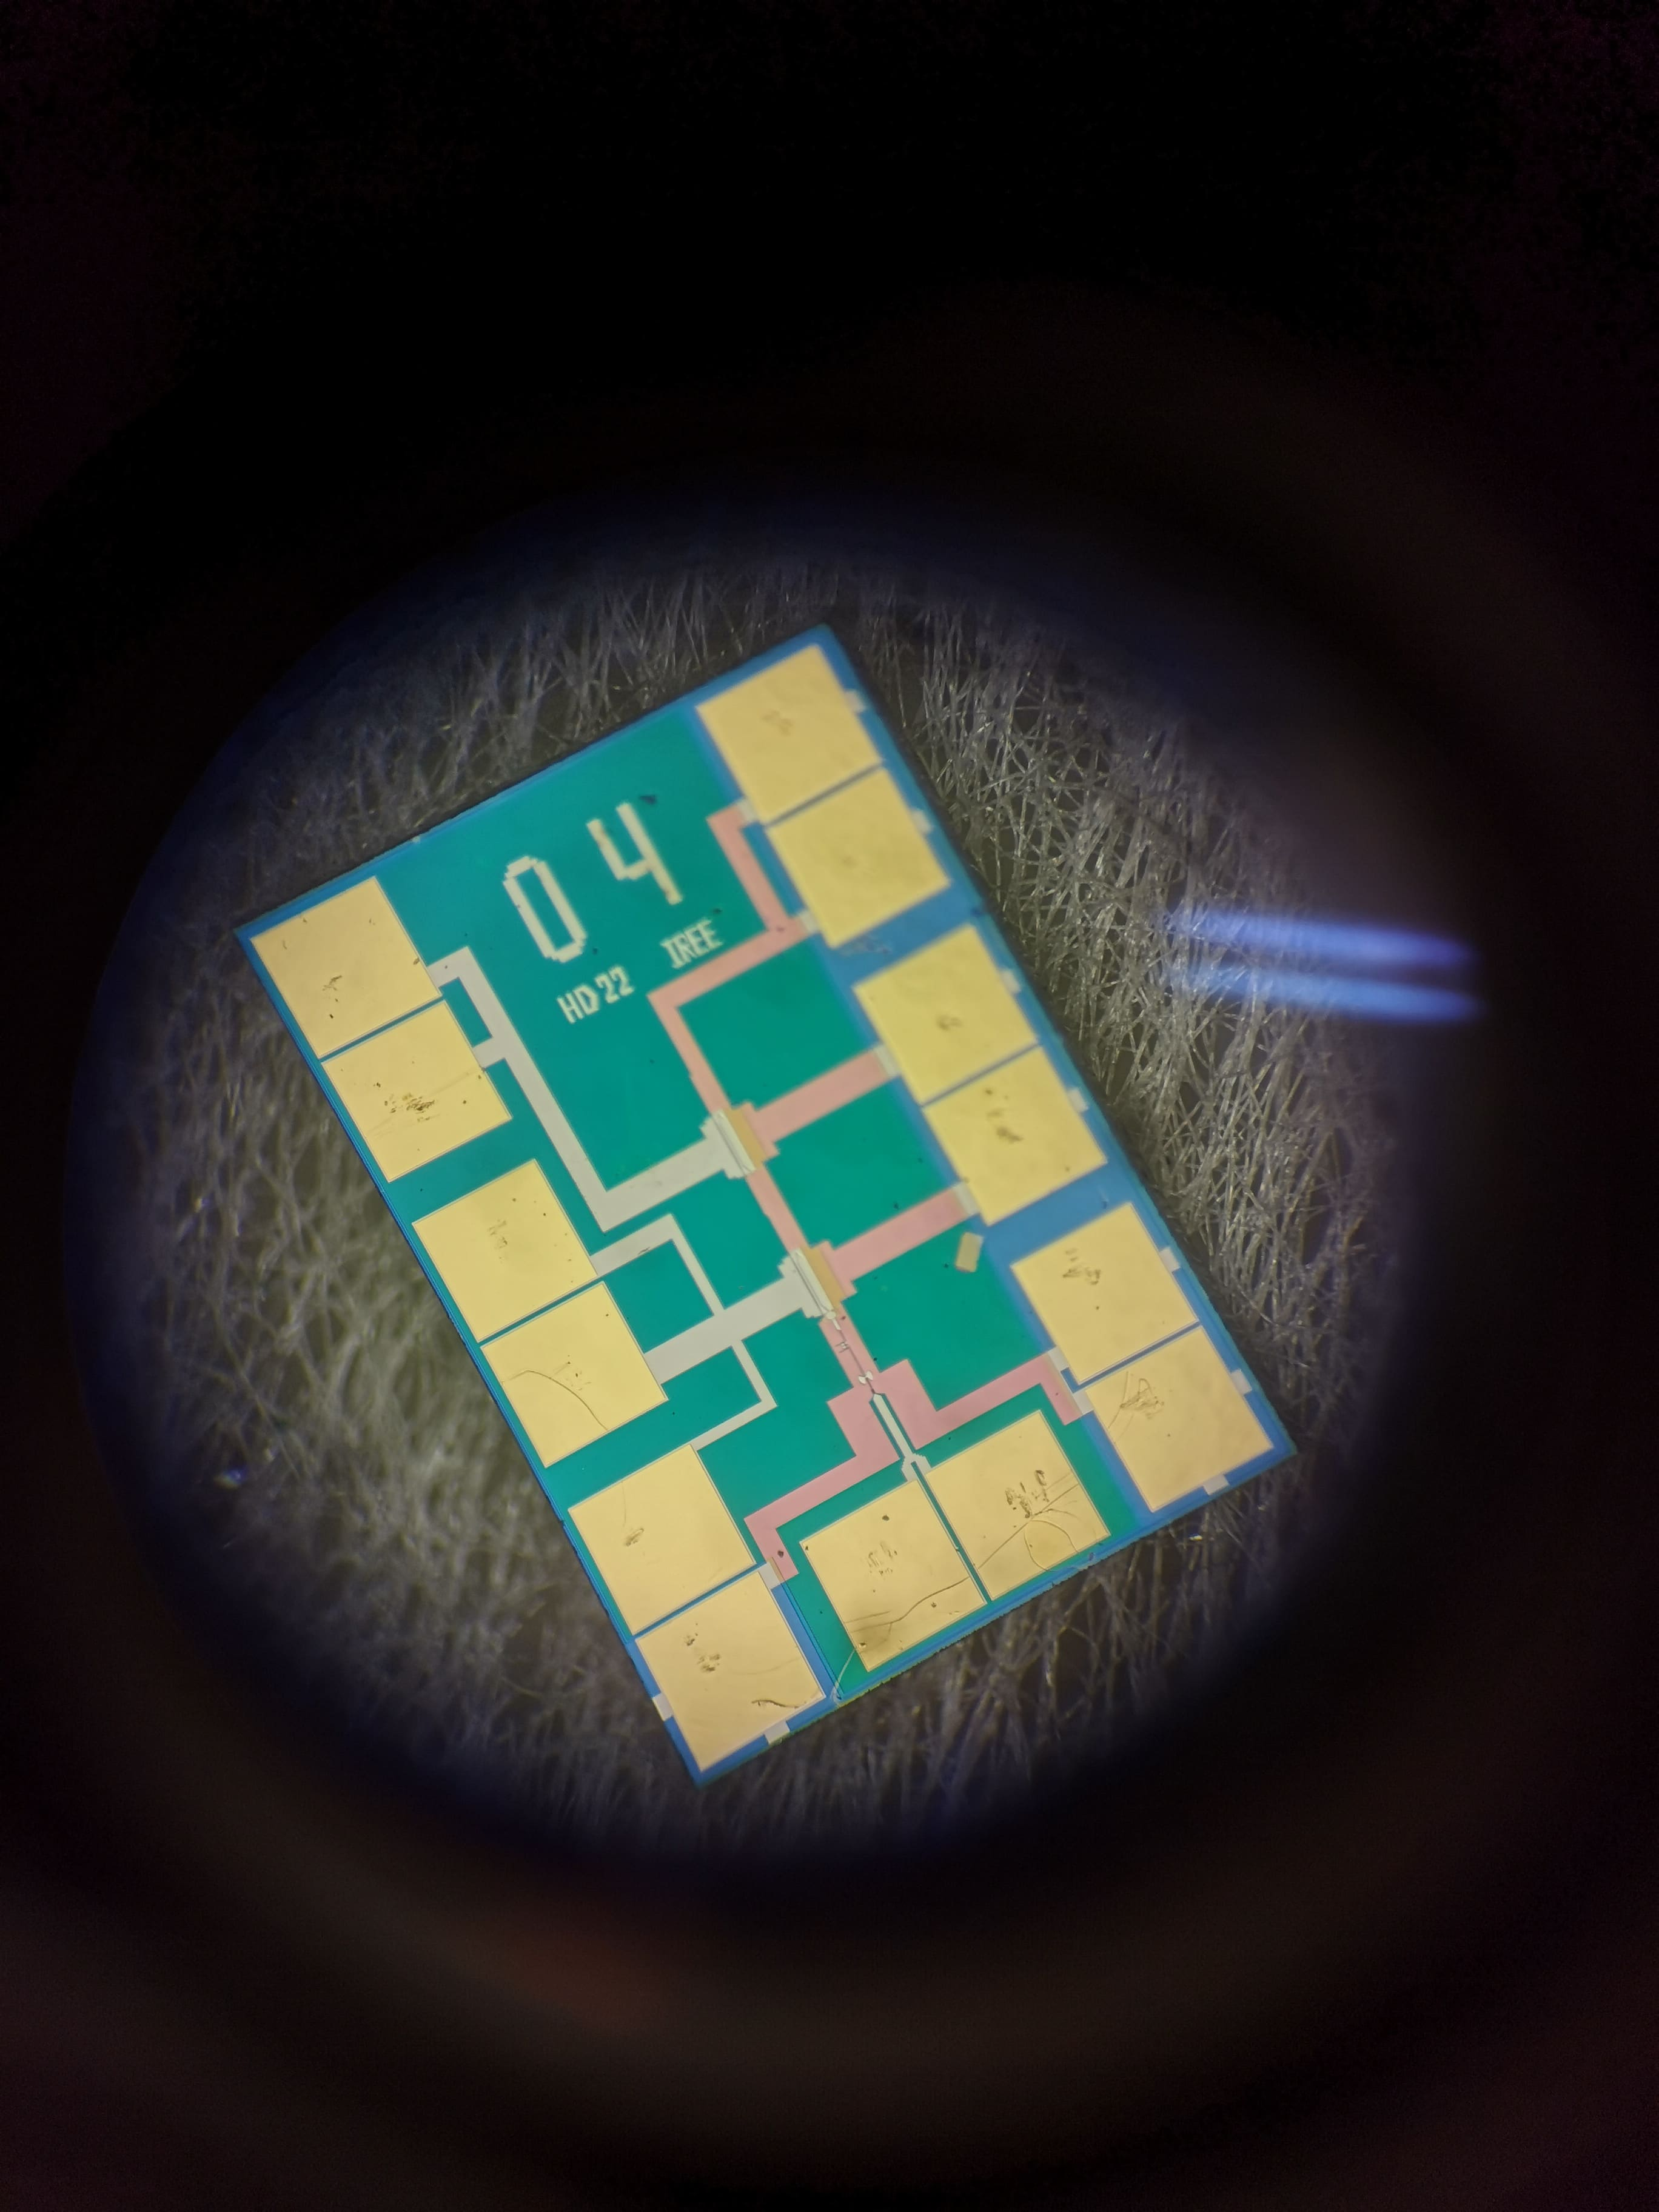
\includegraphics[width=0.85\linewidth]{chip.jpg} \\ a) Фото образца}
    \end{minipage}
    \hfill
    \begin{minipage}[h]{0.5\linewidth}
        \center{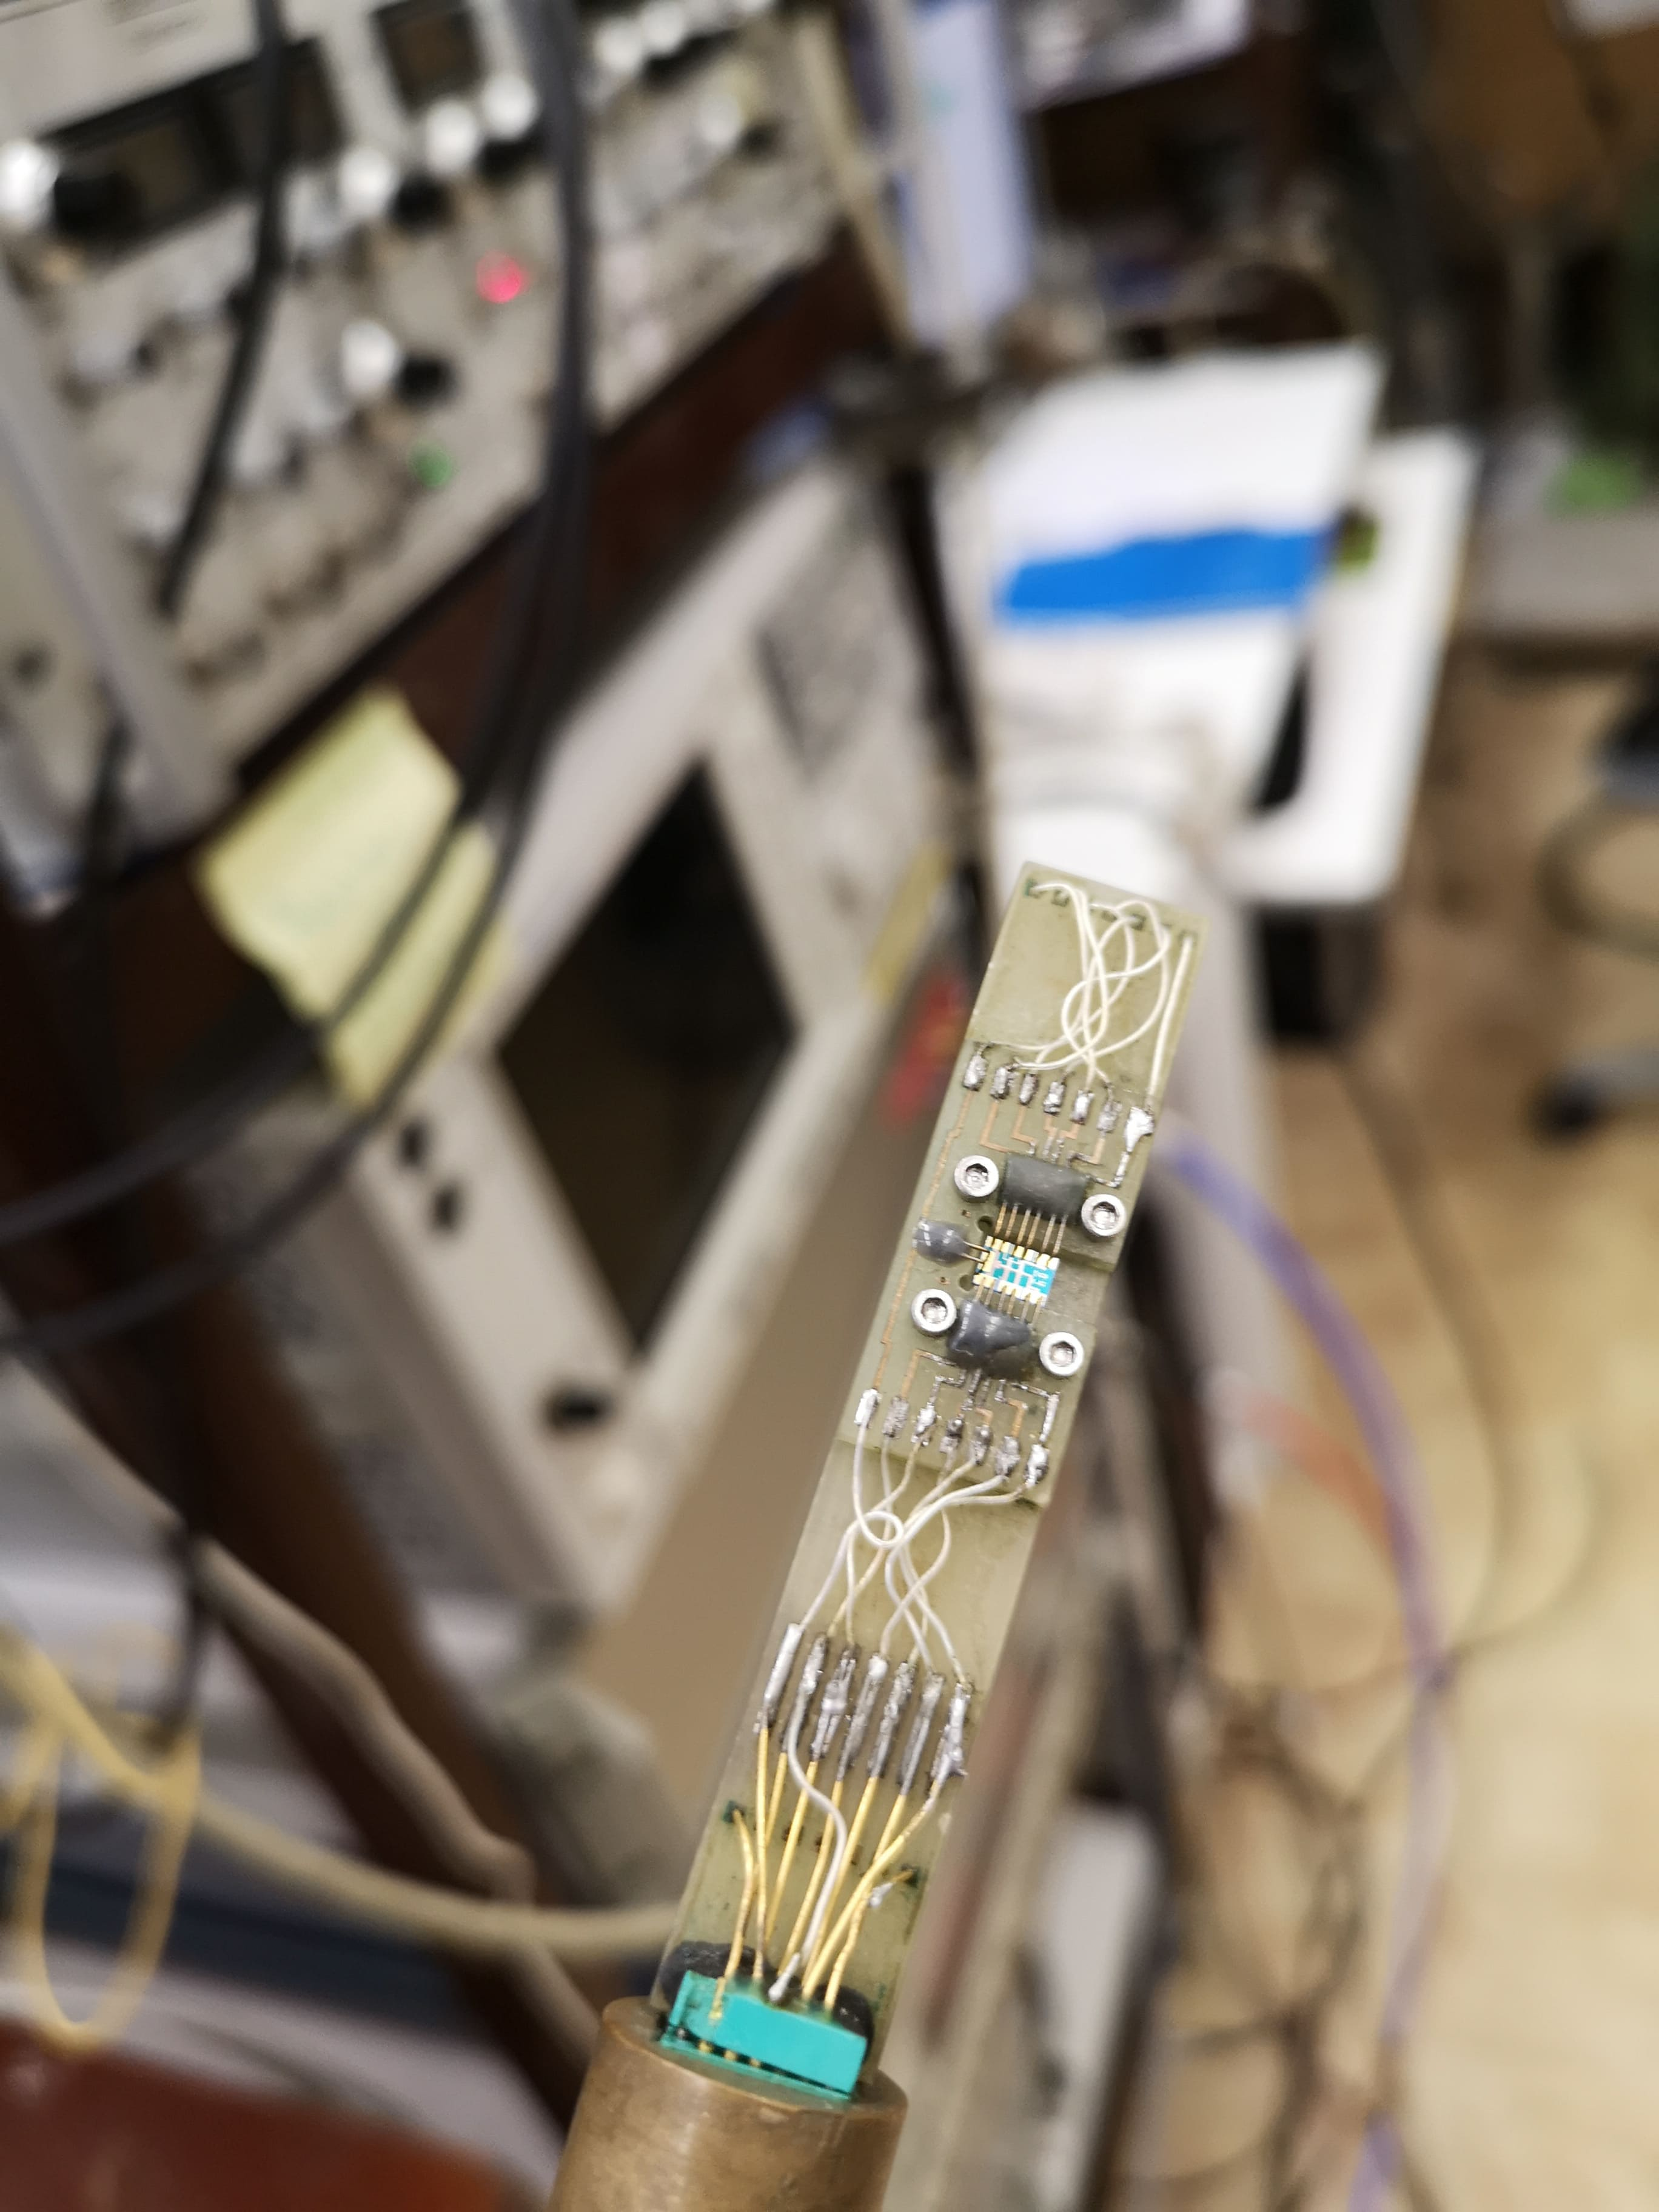
\includegraphics[width=0.85\linewidth]{plata.jpg} \\ б) Держатель с электродами}
    \end{minipage}
    \caption{Исследуемый образец}
    \label{chip}
\end{figure}

\begin{figure}[H]
    \begin{minipage}[h]{0.58\linewidth}
        \center{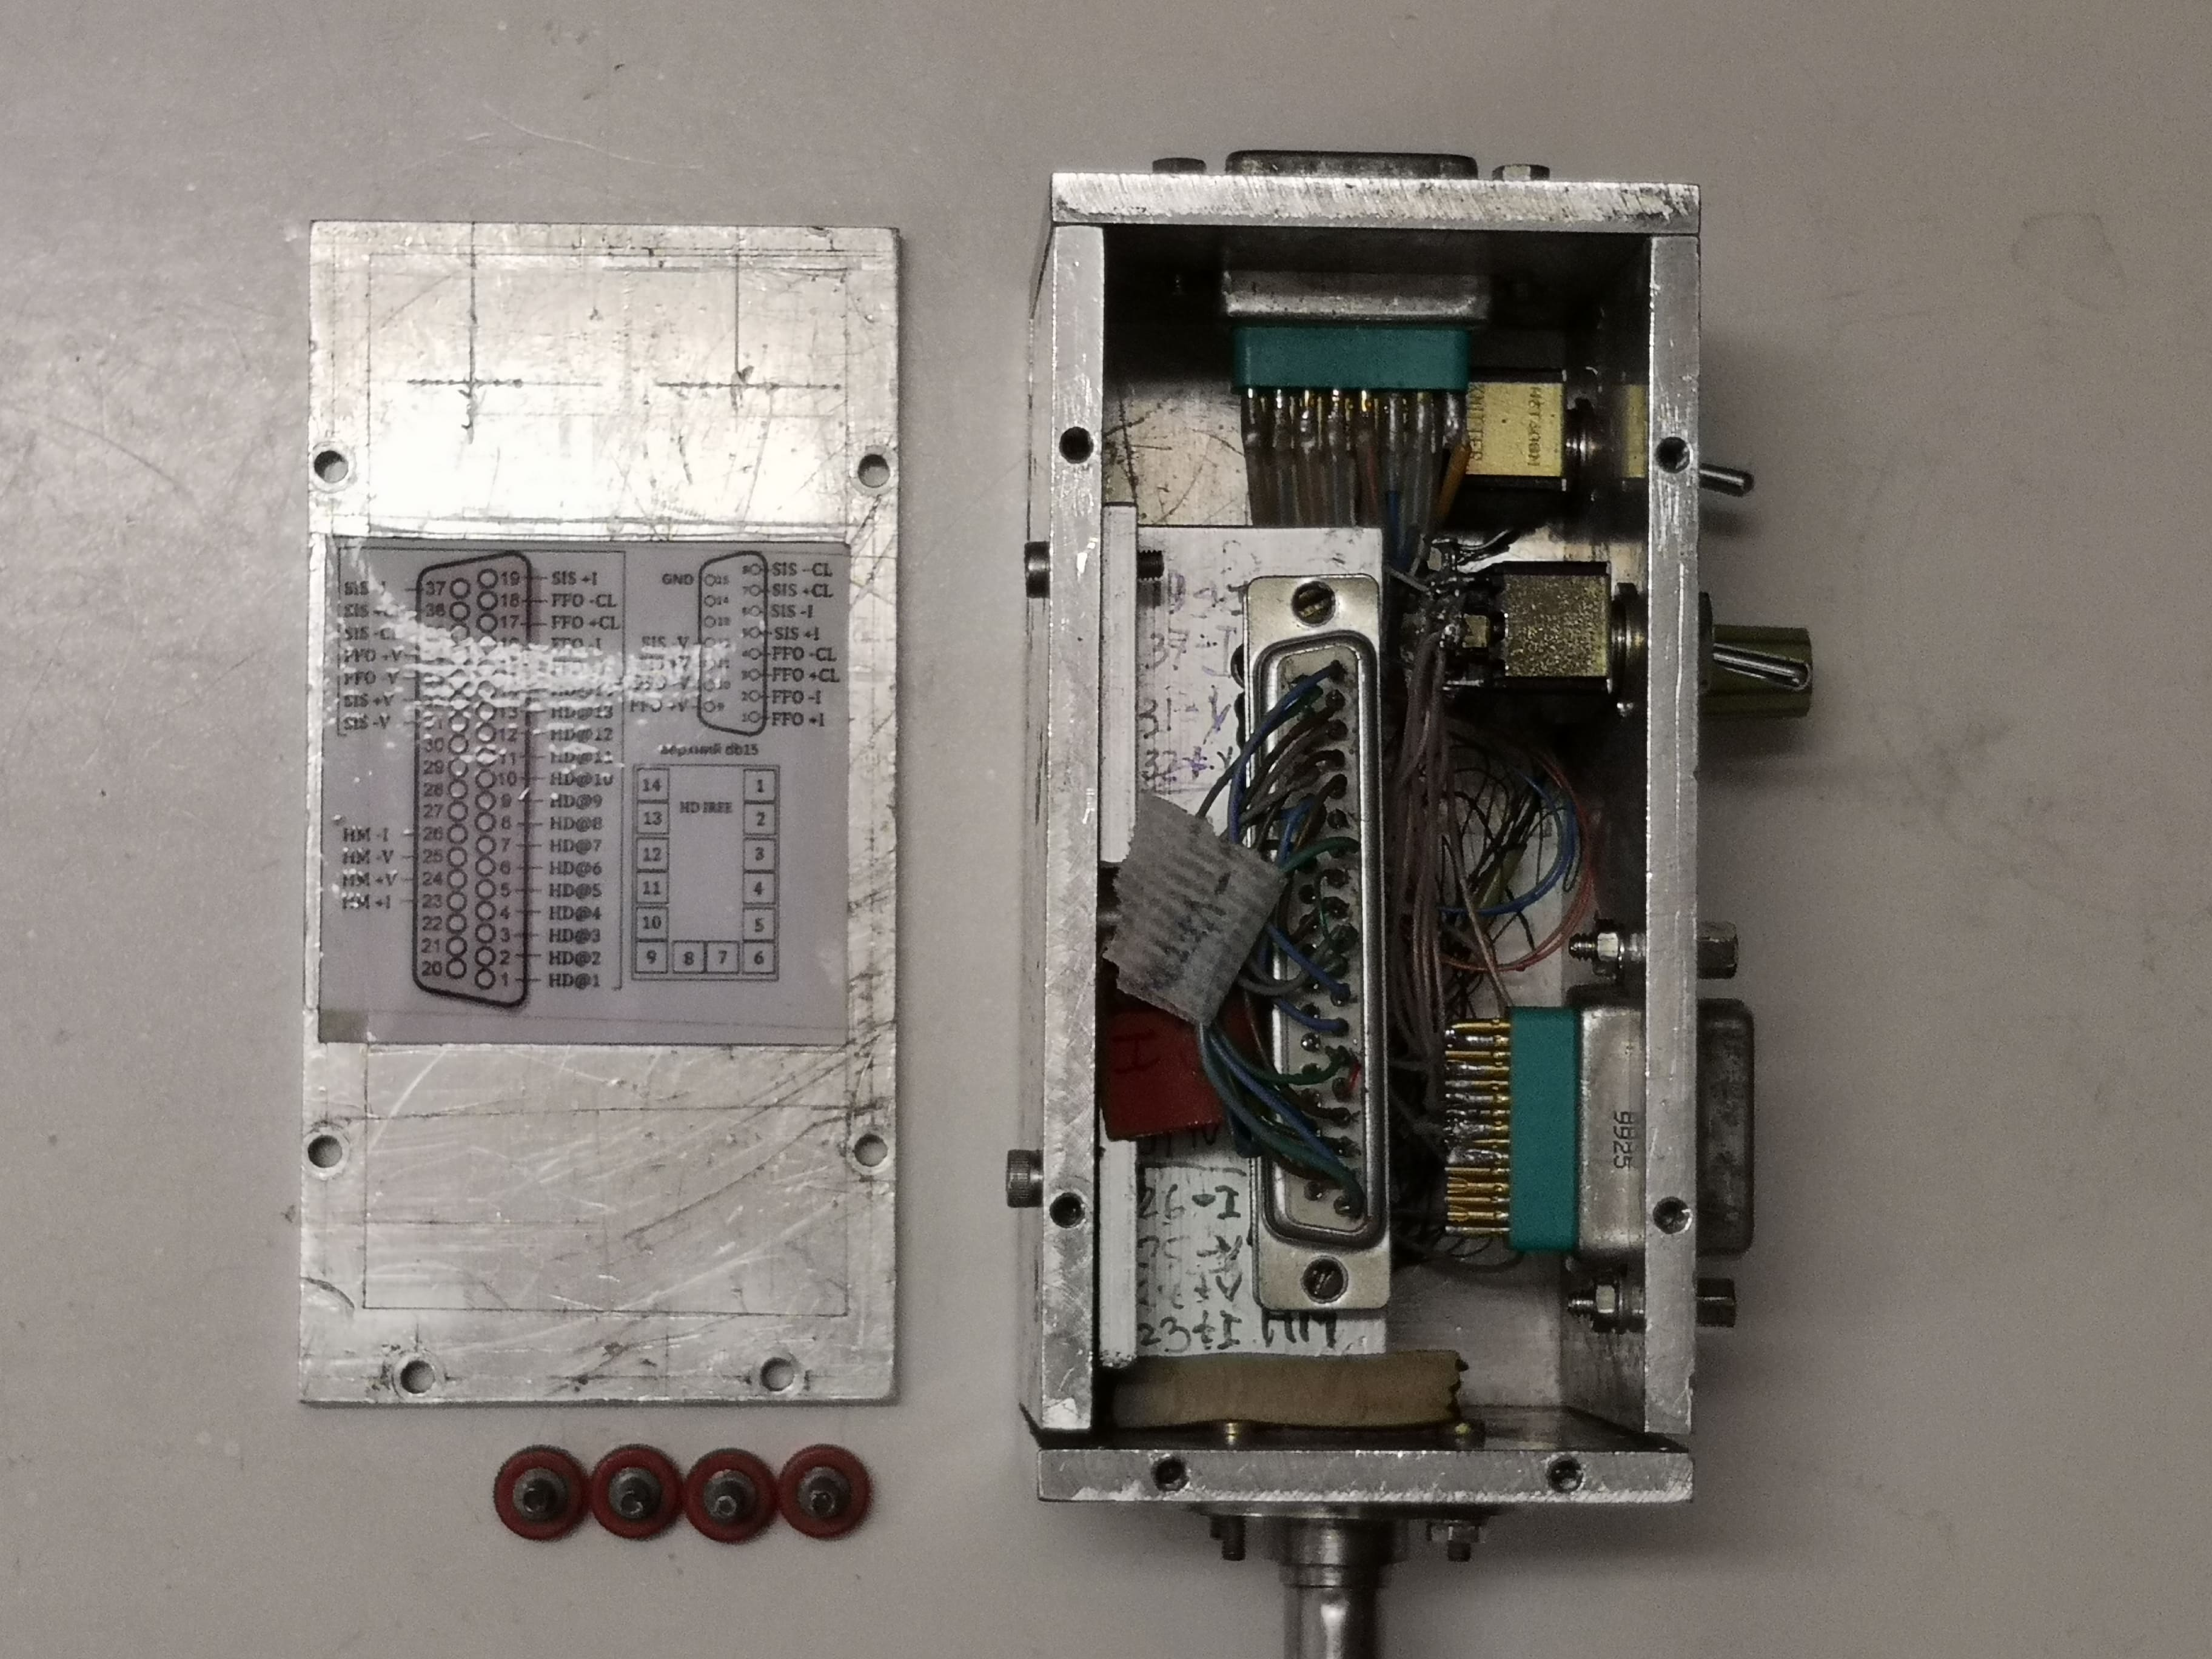
\includegraphics[width=0.92\linewidth]{exp1.jpg} \\ a) Элемент     соединения образца с измерительной установкой}
    \end{minipage}
    \hfill
    \begin{minipage}[h]{0.42\linewidth}
        \center{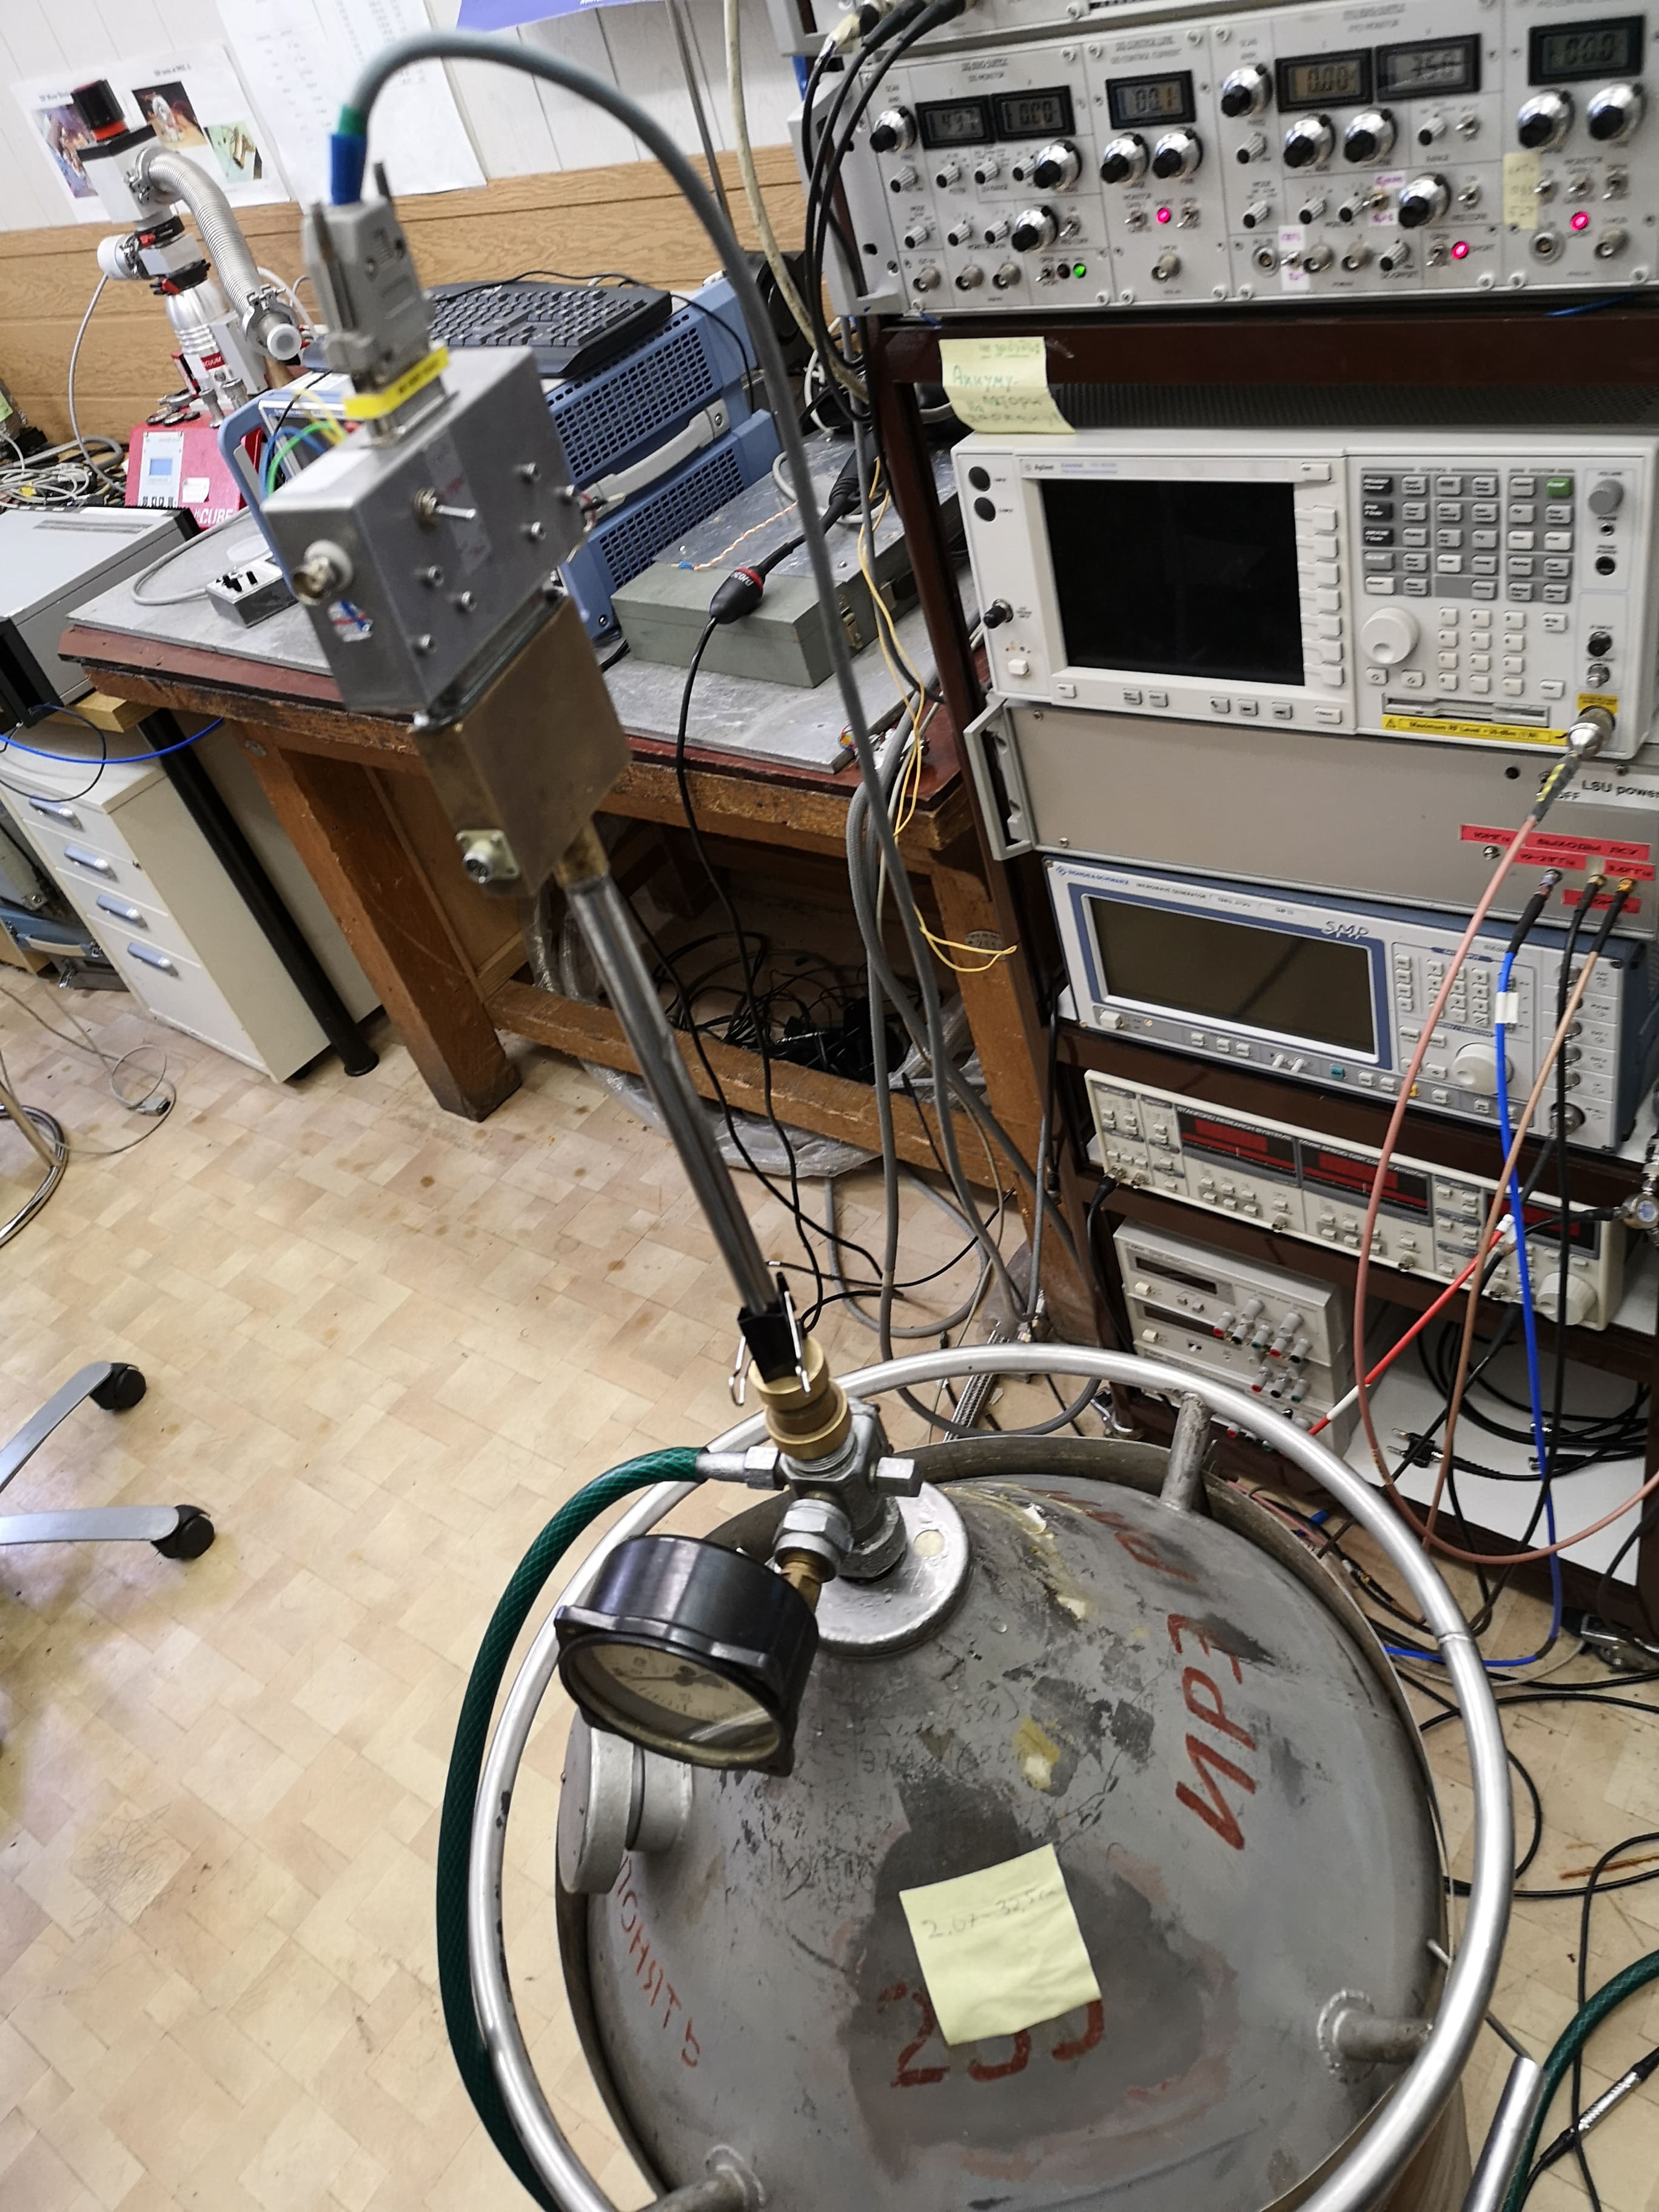
\includegraphics[width=0.92\linewidth]{exp2.jpg} \\ б) Дьюар с опущенным образцом}
    \end{minipage}
    \caption{Исследуемый образец}
    \label{exp}
\end{figure}


\subsection{План}

В рамках работы по исследованию свойств и параметров схем согласования, а также для изучения свойств шунтирования СИС-переходов было поставлено множество опытов с конкретной последовательностью действий:

    \begin{itemize}
        \item выбирается структура, имеющая согласование РДП и СИС (как на рис. \ref{cpl})
        \item подходящий чип подключается нужным образом и опускается охлаждаться в гелий (рис. \ref{exp})
        \item измеряется ВАХ СИС-перехода без воздействия высокочатотного сигнала со стороны РДП, подтверждается исправность детектора
        \item на РДП подаётся наименьшее значение тока смещения, измеряется его ВАХ - на графике появляется первая (слева) кривая, см. рисунок \ref{FFO-exp}\\
        с постоянным шагом увеличивая ток $I_{CL}$, задающий поле, добавляется всё больше кривых на характеристику
        \item параллельно снятию ВАХ на РДП измеряется величина тока накачки на смесителе - она откладывается по тртьей оси (чем краснее цвет точки, тем больше $I_{pump}$)
        \item на ВАХ детектора (рисунок \ref{sis-exp}) появляется несколько накаченных кривых, соответсвующих разным частотам излучения ФФО\\
        выбор значения частоты, для которого записывается очередная кривая, осуществляет измерительный алгоритм
        \item далее ведутся работы по обработке полученных данных, которые не рассматриваются в настоящем обсуждении
    \end{itemize}

\newpage

\subsection{Результаты}

Полученные графики: ВАХ РДП с отложенным по третьей оси относительным значением тока накачки (рисунок \ref{FFO-exp}) и ВАХ СИС с явно выраженными кривыми под воздействием сигнала РДП и без него (рисунок \ref{sis-exp}):

\begin{figure}[H]
    \centering
    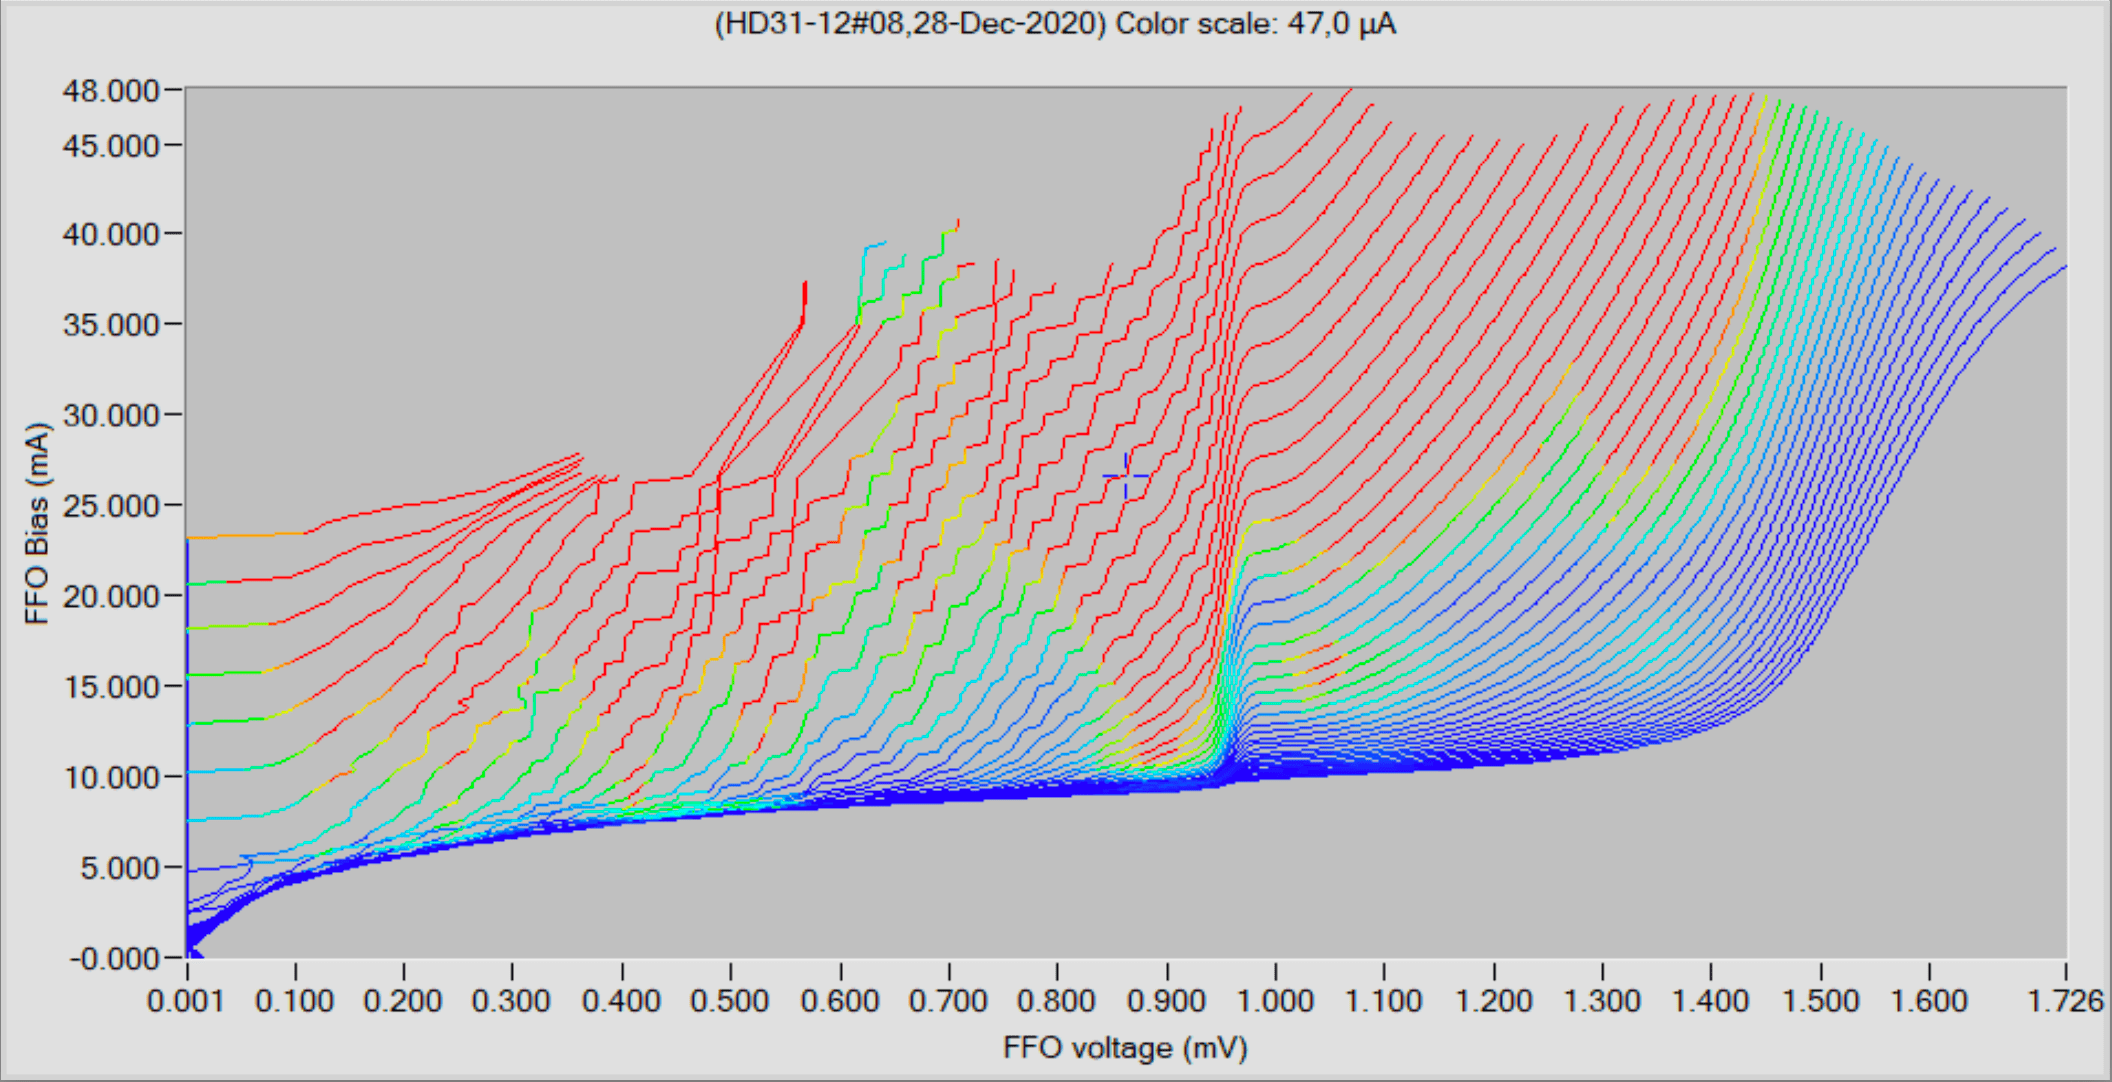
\includegraphics[scale = 1.15]{FFO-exp.png}
    \caption{ВАХ РДП}
    \label{FFO-exp}
\end{figure}

\begin{figure}[H]
    \centering
    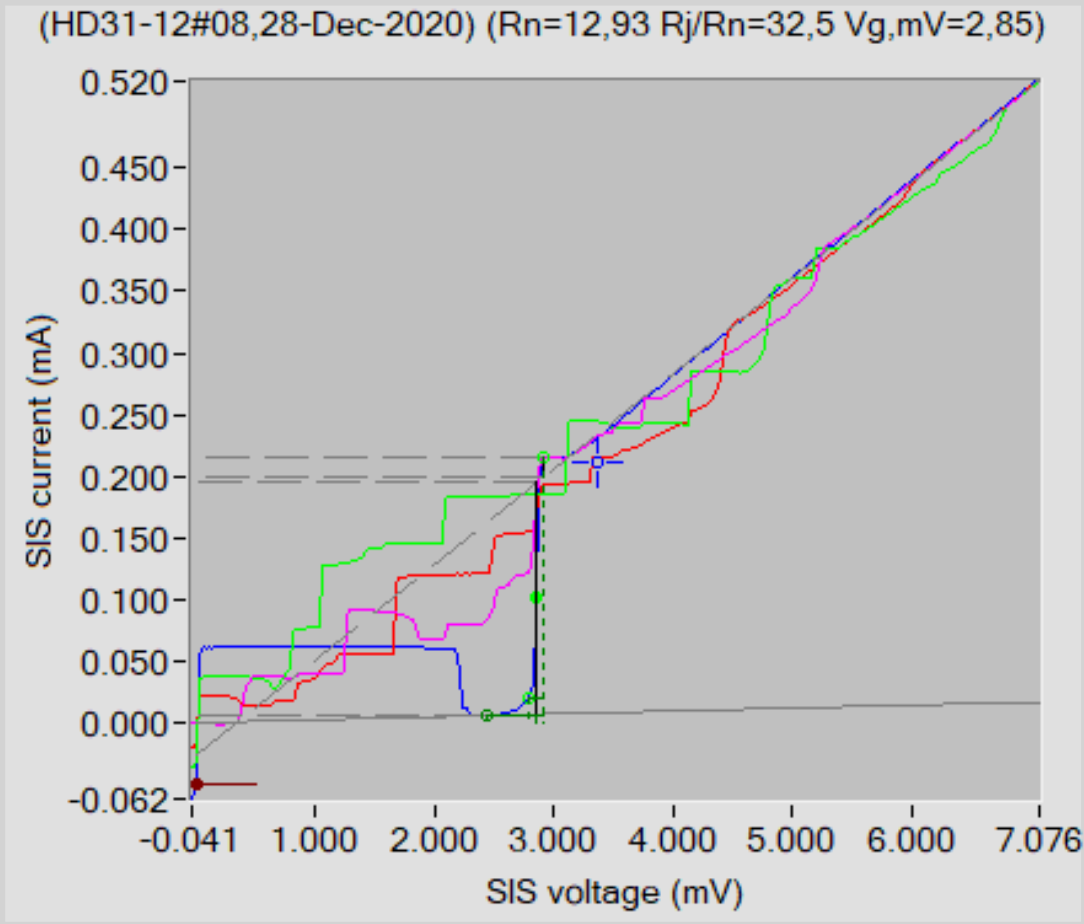
\includegraphics[scale = 1.7]{sis-exp.png}
    \caption{ВАХ СИС}
    \label{sis-exp}
\end{figure}

\begin{center}
    \textit{Ступень на малых напряжениях исходной кривой (без накачки, син.) связана с эффектами крит.тока и не является результатом воздействия СВЧ сигнала от РДП}
\end{center}

\newpage

\section{Выводы}

В ходе проделанной работы мы получили следующие результаты:

    \begin{itemize}
        \item краткое введение в физику джозефсоновский переходов;
        \item описание принципов и целей гетеродинирования;
        \item поверхностное описание работы РДП:
                \begin{itemize}
                    \item принцип генерации СВЧ сигнала;
                    \item режим ступеней Фиске;
                    \item режим флакс-флоу;
                    \item процесс накачки СИС-детектора;
                \end{itemize}
        \item данные, полученные в одном из поставленных экспериментов.
    \end{itemize}

По полученным эксперементальным данным можно судить о том, что изложенная теория отлично воплощена на практике, исследуемые образцы обладают ожидаемым функционалом и полностью готовы к использованию в тех или иных целях.

\newpage

\begin{thebibliography}{7}
        \bibitem{Shmidt}
        Шмидт В.В., Введение в физику сверхпроводников, М.: МЦНМО, 2000
        \bibitem{Likharev}
        Лихарёв К.В., Введение в динамику джозефсоновских переходов, М.: Наука, 1985
        \bibitem{Tucker}
        Tucker J.R., Feldman M.J., Quantum detection at millimeter wavelengths, New York: Reviews of Modern Physics, 1985
        \bibitem{Barychev}
        Barychev A.M, SIS THz mixer integrated with a superconducting FFO,  GrafiMedia Groningen: Bedrijf RuG, 2005
        \bibitem{Kinev}
        Кинёв Н.В., Генерация и прием ТГц излучения с использованием сверхповодниковых интегральных устройств, М.: МФТИ, 2012
        \bibitem{Glazkov}
        Глазков В.Н., Энергетические диаграммы для квазичастотного тока в контактах сверхпроводников. Эффект Джозефсона., М.: МФТИ, 2017
        \bibitem{Atepalikhin}
        Атепалихин А.А., Туннелирование электронов через потенциальный барьер. Контакты типа NIN, SIN, SIS, М.: МФТИ, 2021
\end{thebibliography}

\end{document}